\chapter{Results and Performance Analysis}
\label{Chapter5}

This chapter presents a comprehensive analysis of our experimental results comparing the Lion and AdamW optimizers for cross-encoder reranking models. We evaluate three distinct transformer architectures (MiniLM, GTE, and ModernBERT) across multiple metrics and examine their training dynamics through detailed visualizations.

\section{Experimental Results}

\subsection{Main Performance Metrics}

Table~\ref{tab:main_results} presents the comprehensive evaluation results for all model configurations on both the TREC 2019 Deep Learning Track and MS MARCO development set. The results are tracked across three training epochs for each model-optimizer combination.

\begin{table}[htbp]
\centering
\caption{Evaluation Results on TREC-DL 2019 and MS-MARCO Dev Passage Ranking}
\label{tab:main_results}
\begin{tabular}{l l c c c c c}
\toprule
\textbf{Model} & \textbf{Optimizer} & \textbf{NDCG@10} & \textbf{MAP} & \textbf{MRR@10} & \textbf{R-Prec} & \textbf{P@10} \\
\midrule
MiniLM & AdamW & 0.7127 & 0.4908 & 0.5826 & 0.4962 & 0.8023 \\
MiniLM & Lion & 0.6808 & 0.4706 & \textbf{0.5988} & 0.4923 & 0.8023 \\
GTE & AdamW & 0.7224 & 0.5005 & 0.5940 & 0.4957 & 0.8140 \\
GTE & Lion & 0.6909 & 0.4921 & 0.5957 & 0.5053 & 0.8140 \\
ModernBERT & AdamW & 0.7105 & 0.5066 & 0.5865 & 0.5161 & 0.8163 \\
ModernBERT & Lion & \textbf{0.7225} & \textbf{0.5115} & 0.5907 & \textbf{0.5183} & \textbf{0.8209} \\
\bottomrule
\end{tabular}
\end{table}

\subsection{Training Dynamics Analysis}

To better understand the behavior of each optimizer-model combination, we analyze their training dynamics through various metrics. The following figures present comparative visualizations of training trajectories.

\subsubsection{ModernBERT Training Dynamics}

\begin{figure}[htbp]
    \centering
    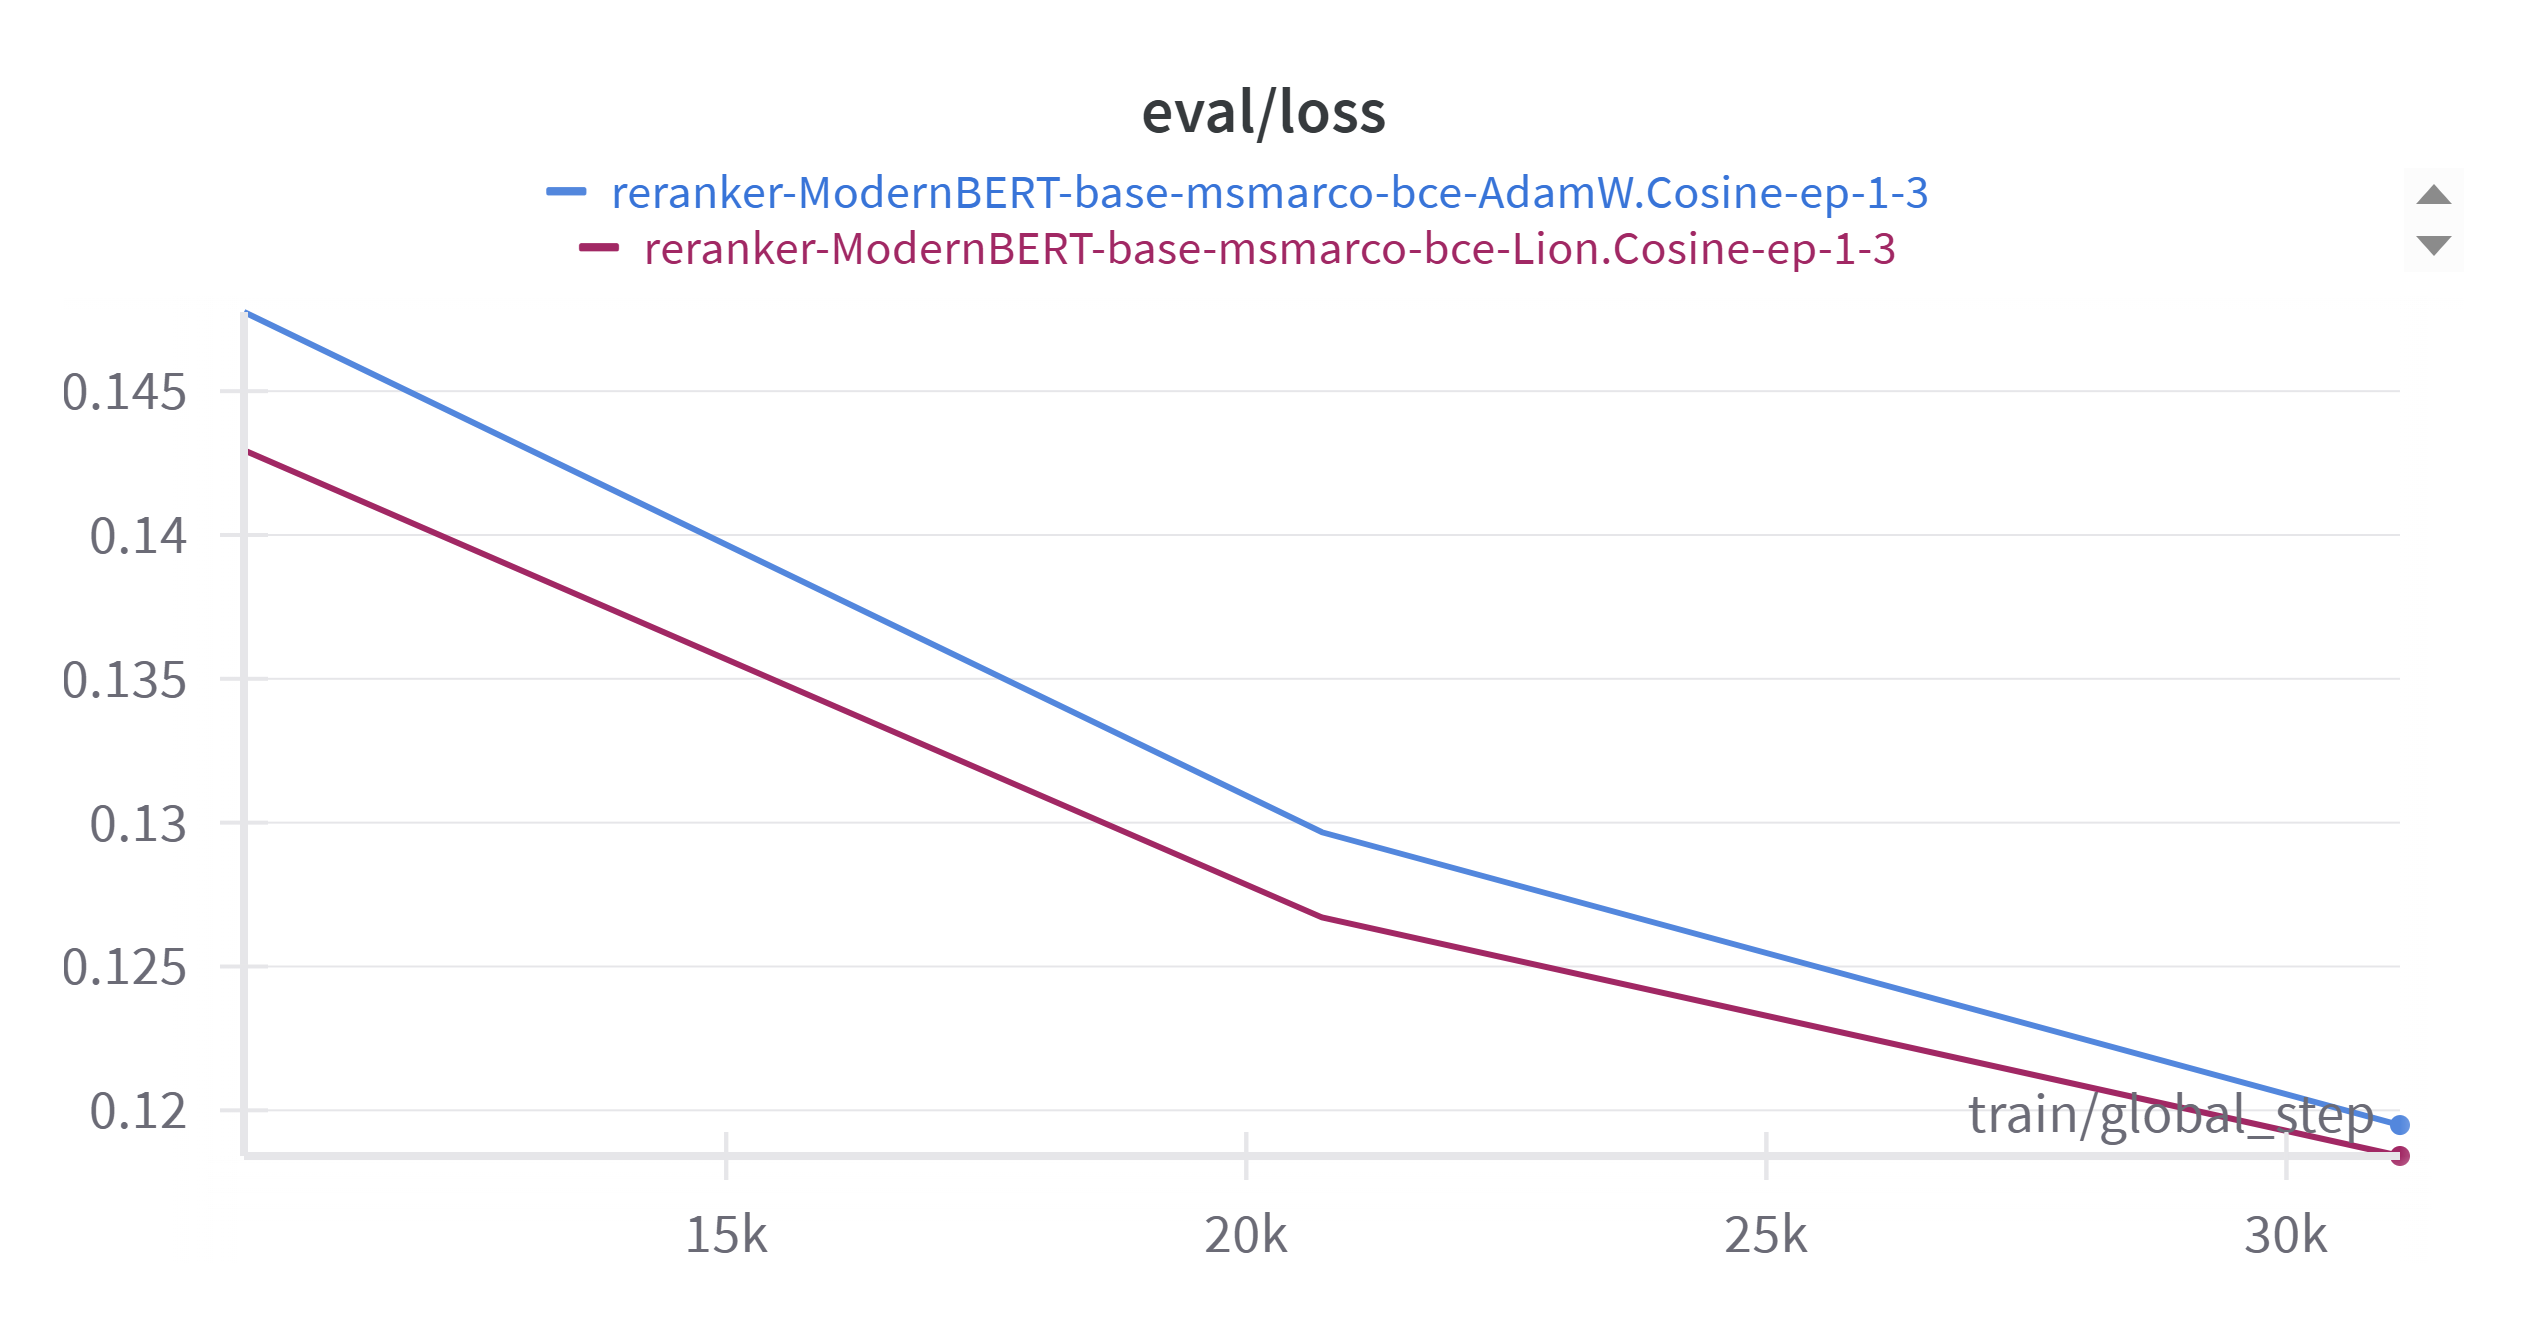
\includegraphics[width=0.8\textwidth]{Figures/modernBERT-Lion-AdamW-eval_loss.png}
    \caption{ModernBERT: Evaluation Loss Comparison between Lion and AdamW}
    \label{fig:modernbert_eval_loss}
\end{figure}

\begin{figure}[htbp]
    \centering
    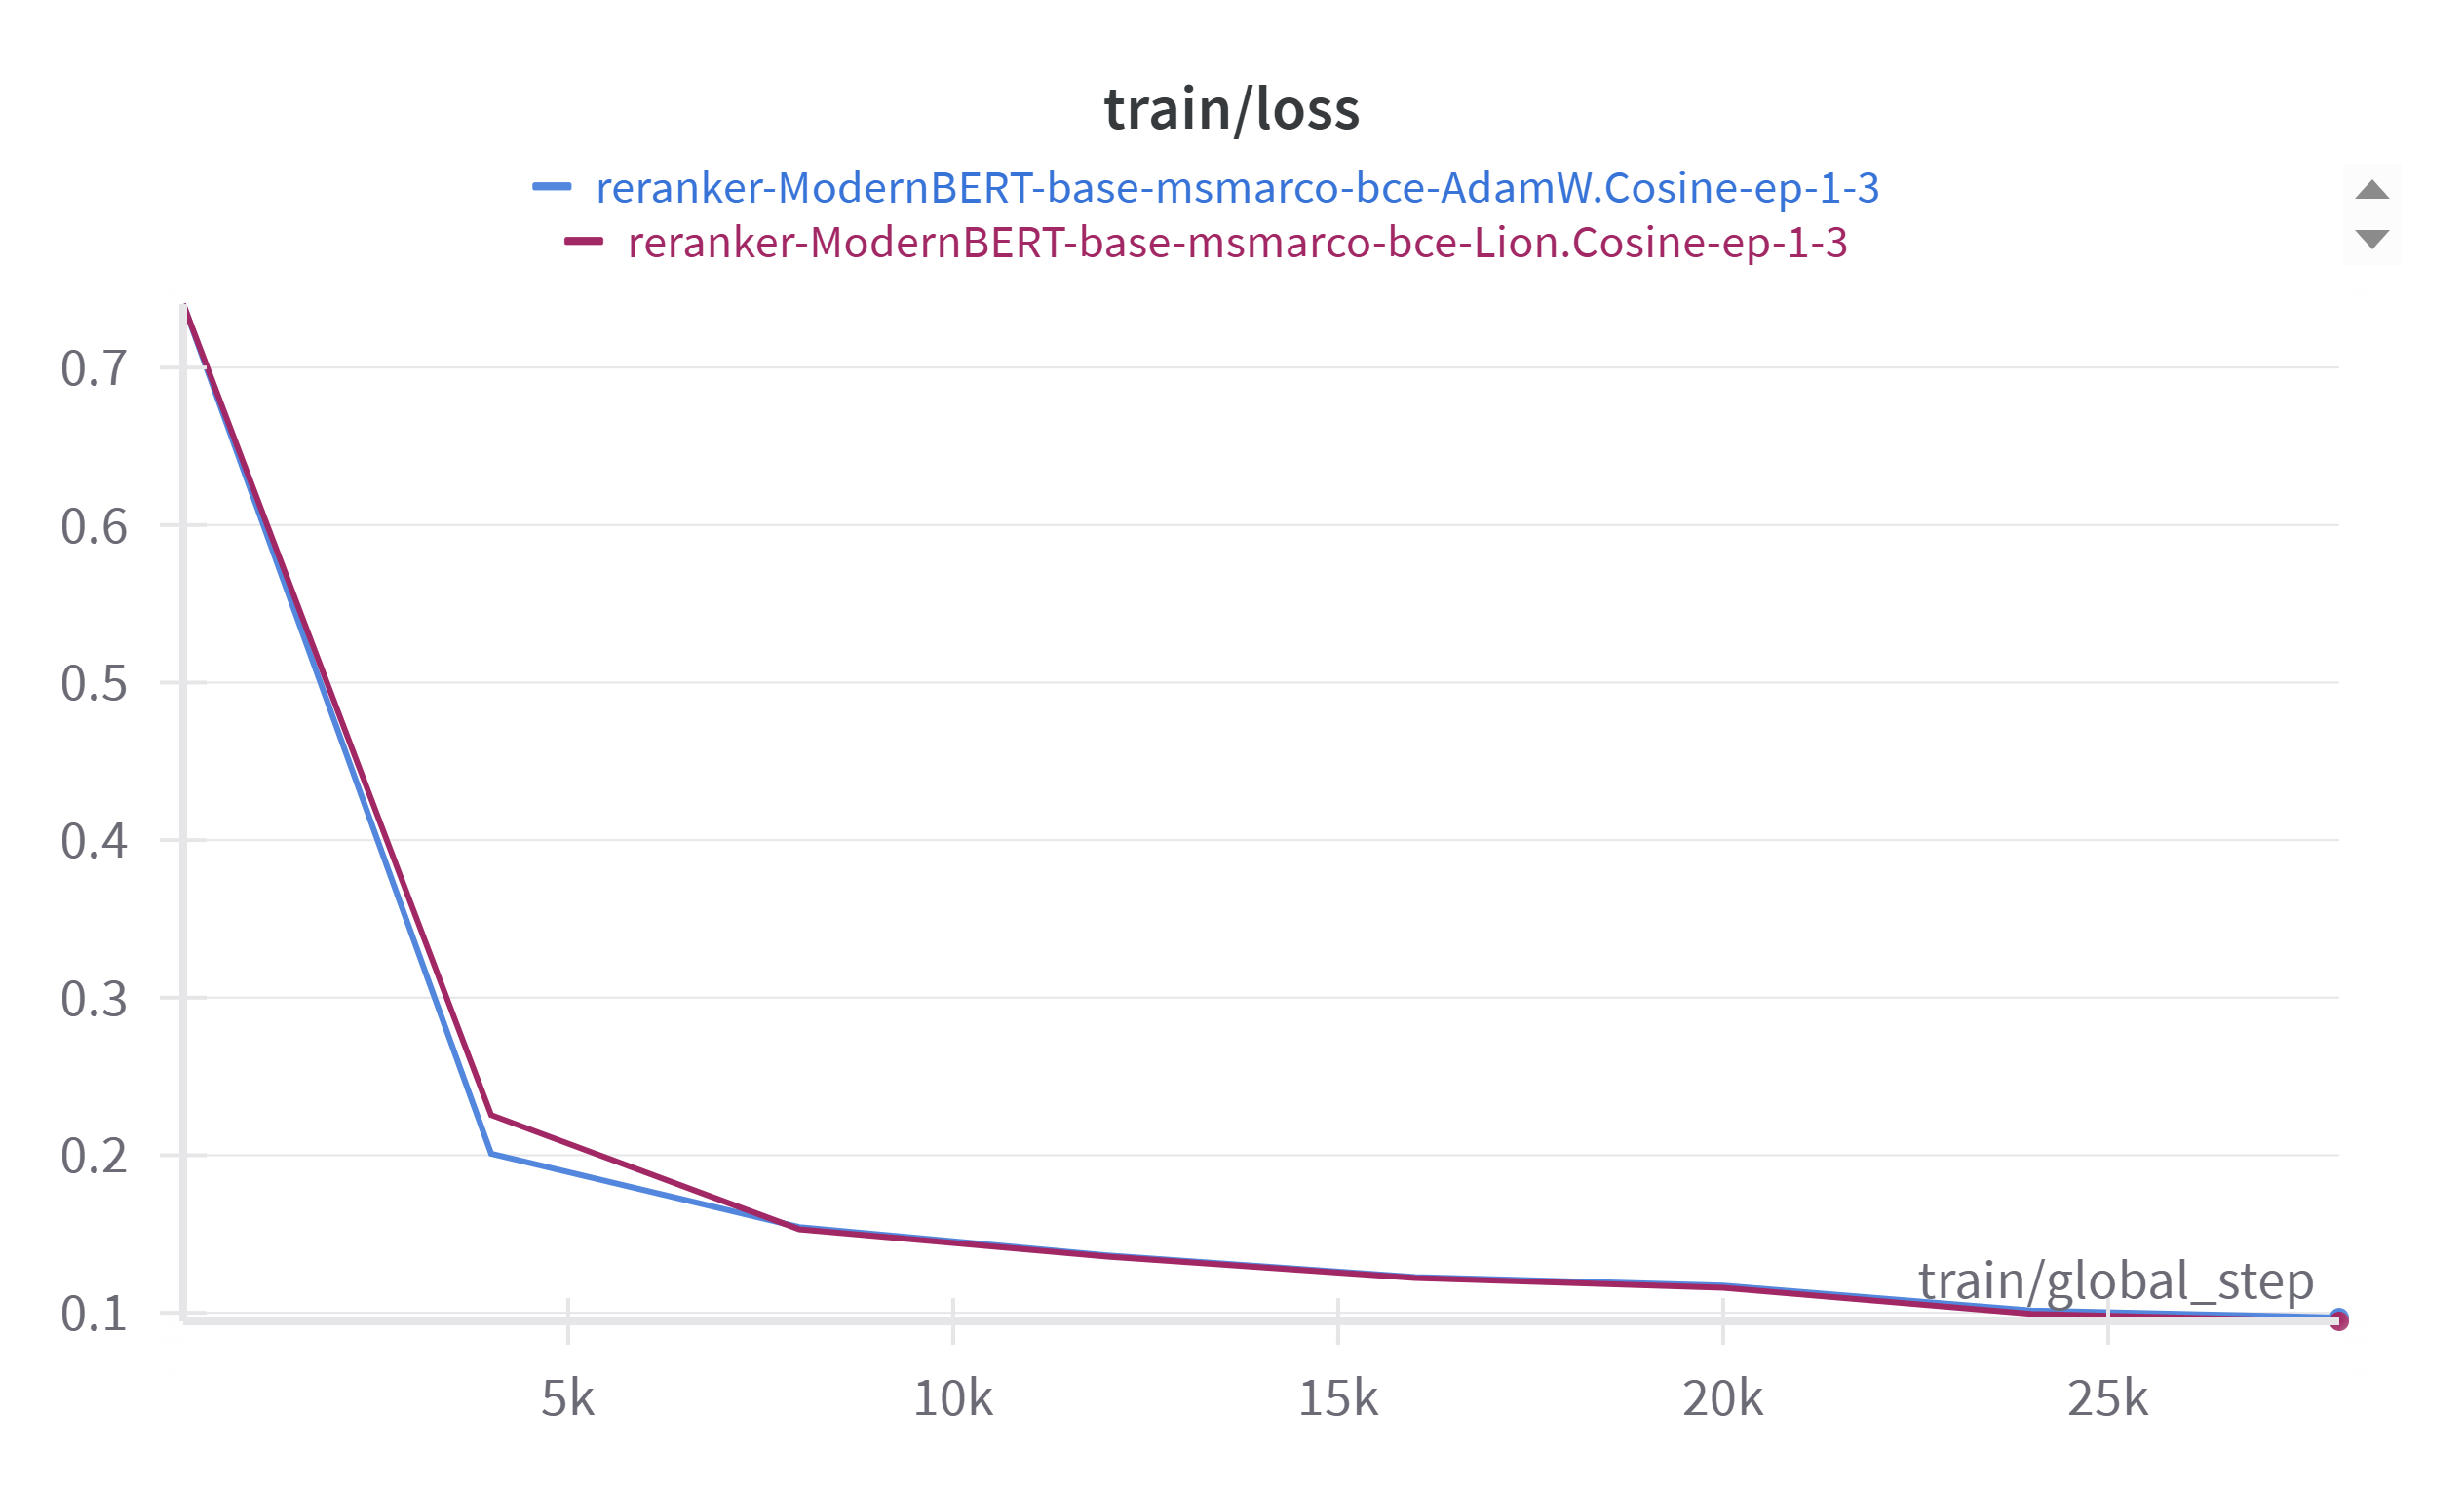
\includegraphics[width=0.8\textwidth]{Figures/modernBERT-Lion-adamW-train_loss.png}
    \caption{ModernBERT: Training Loss Progression}
    \label{fig:modernbert_train_loss}
\end{figure}

\begin{figure}[htbp]
    \centering
    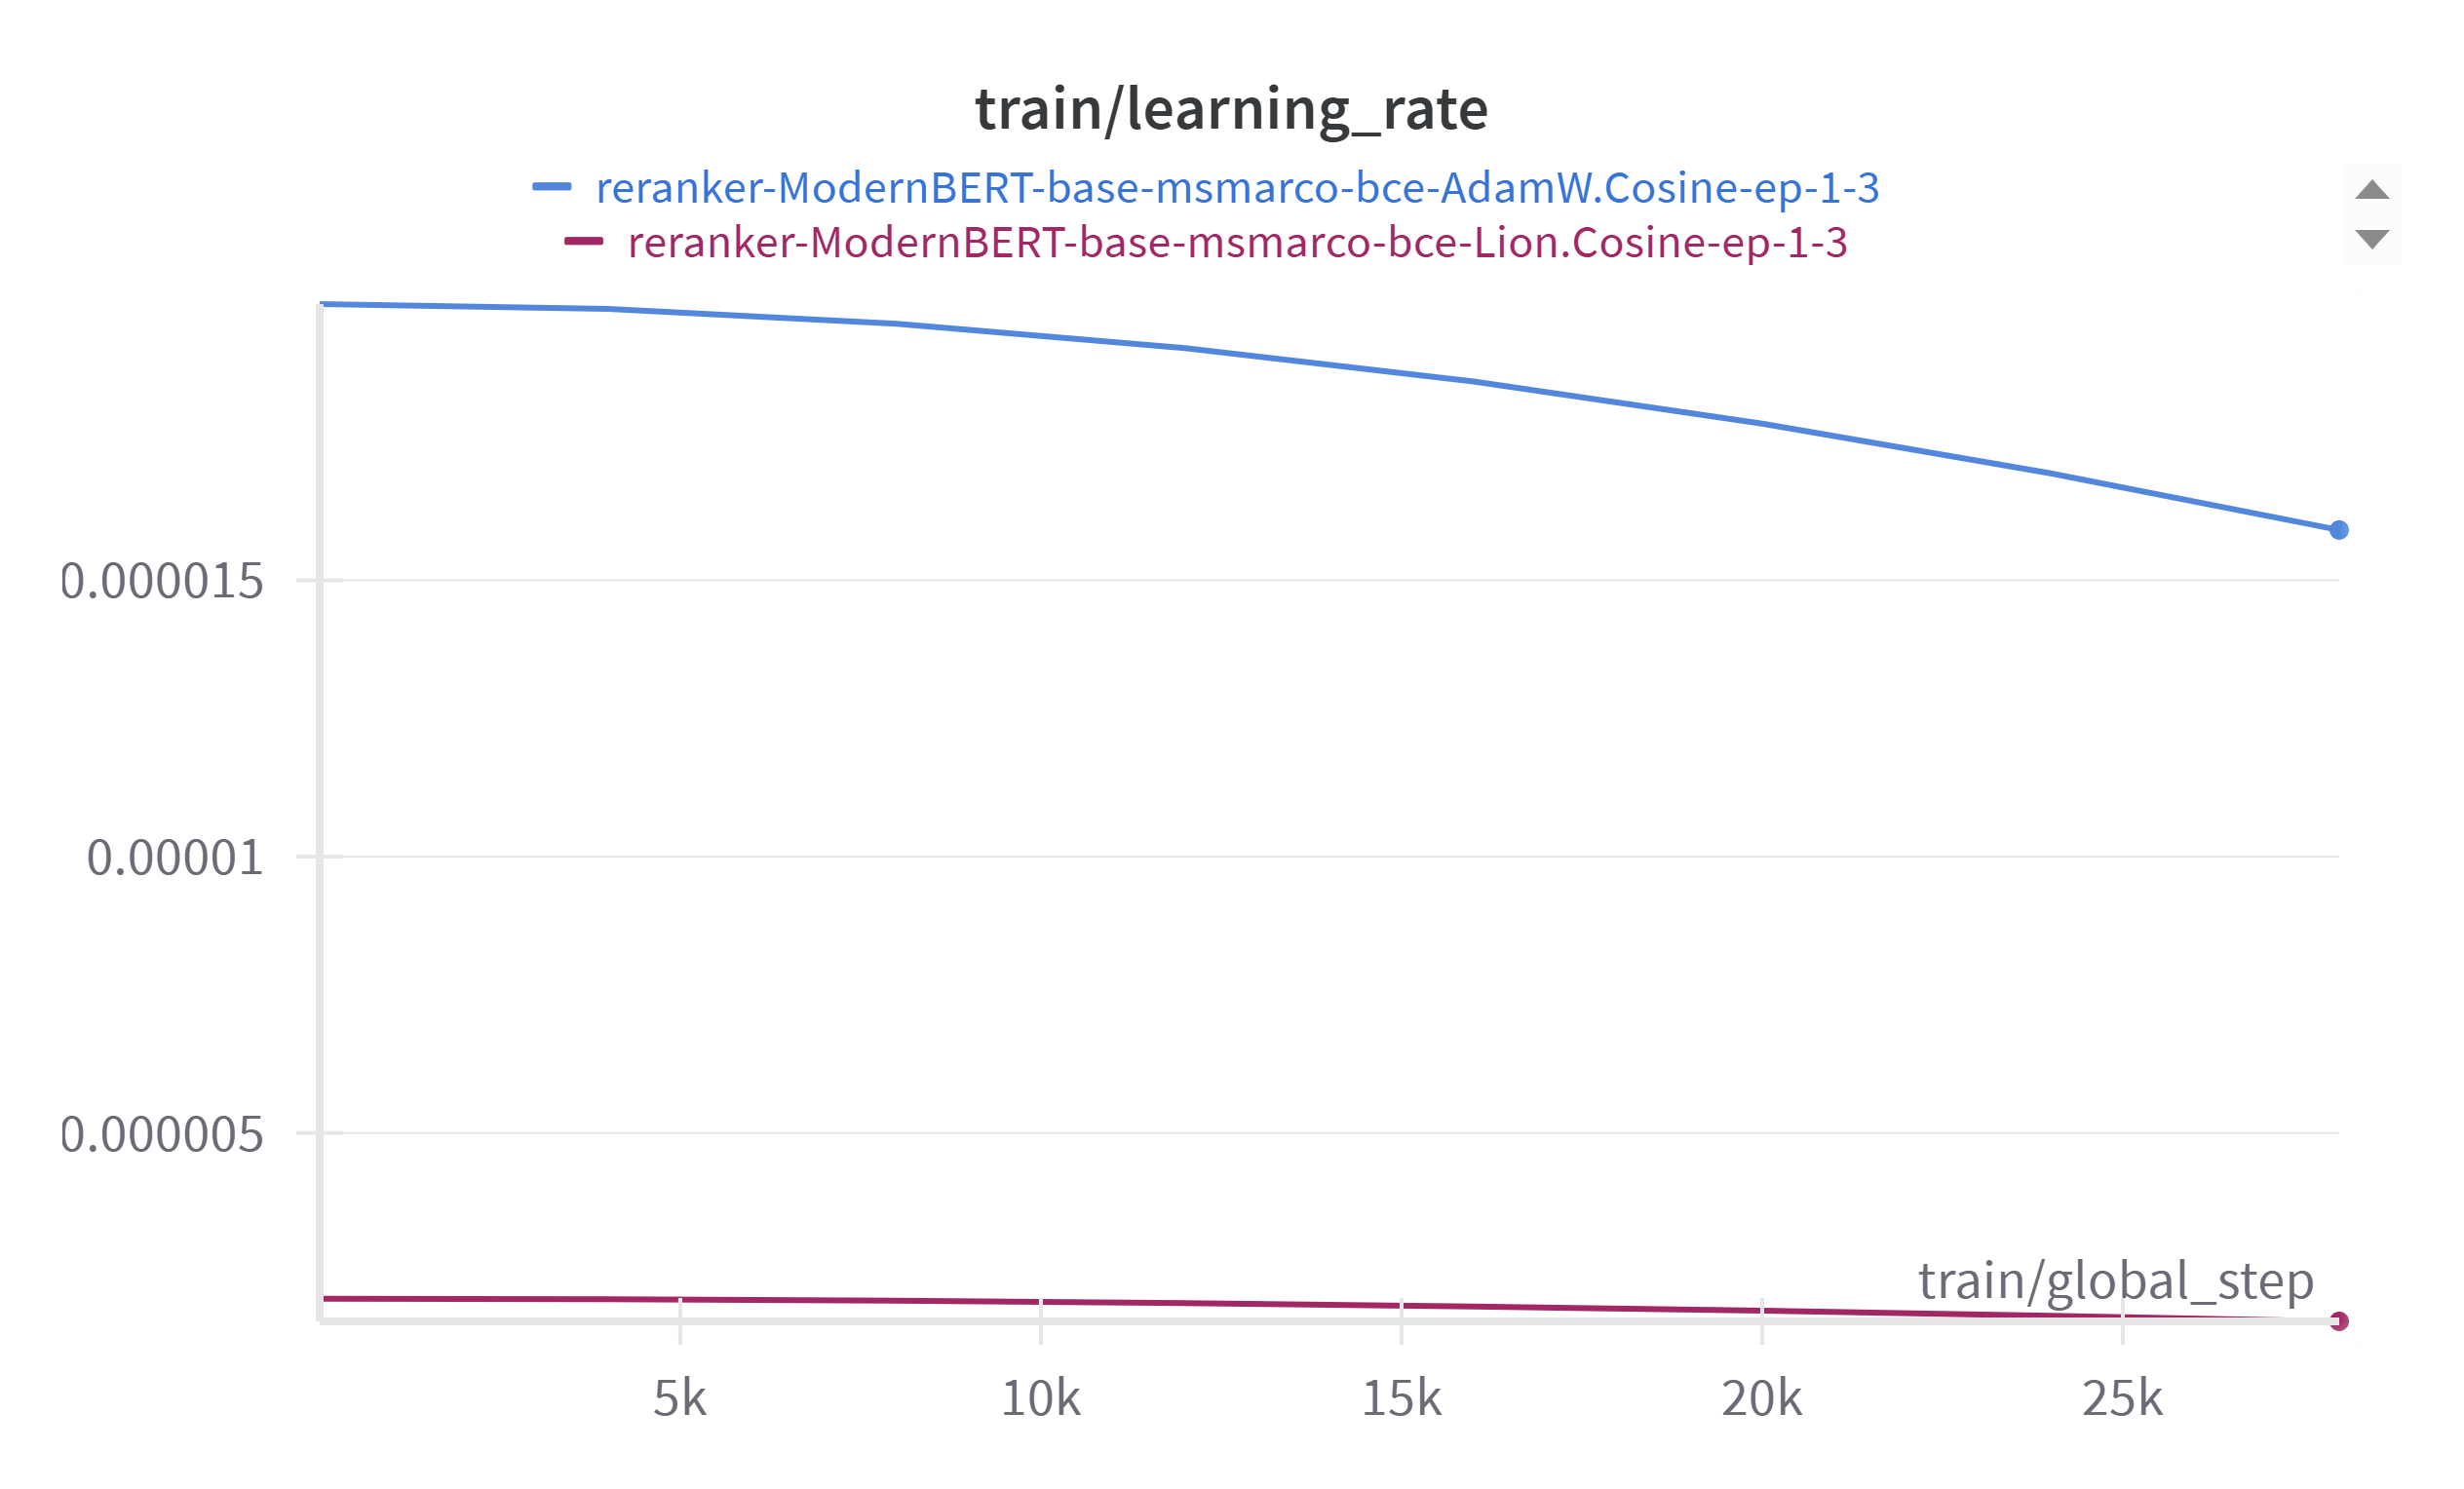
\includegraphics[width=0.8\textwidth]{Figures/modernBERT-Lion-adamW-lrate.png}
    \caption{ModernBERT: Learning Rate Schedule}
    \label{fig:modernbert_lr}
\end{figure}

\begin{figure}[htbp]
    \centering
    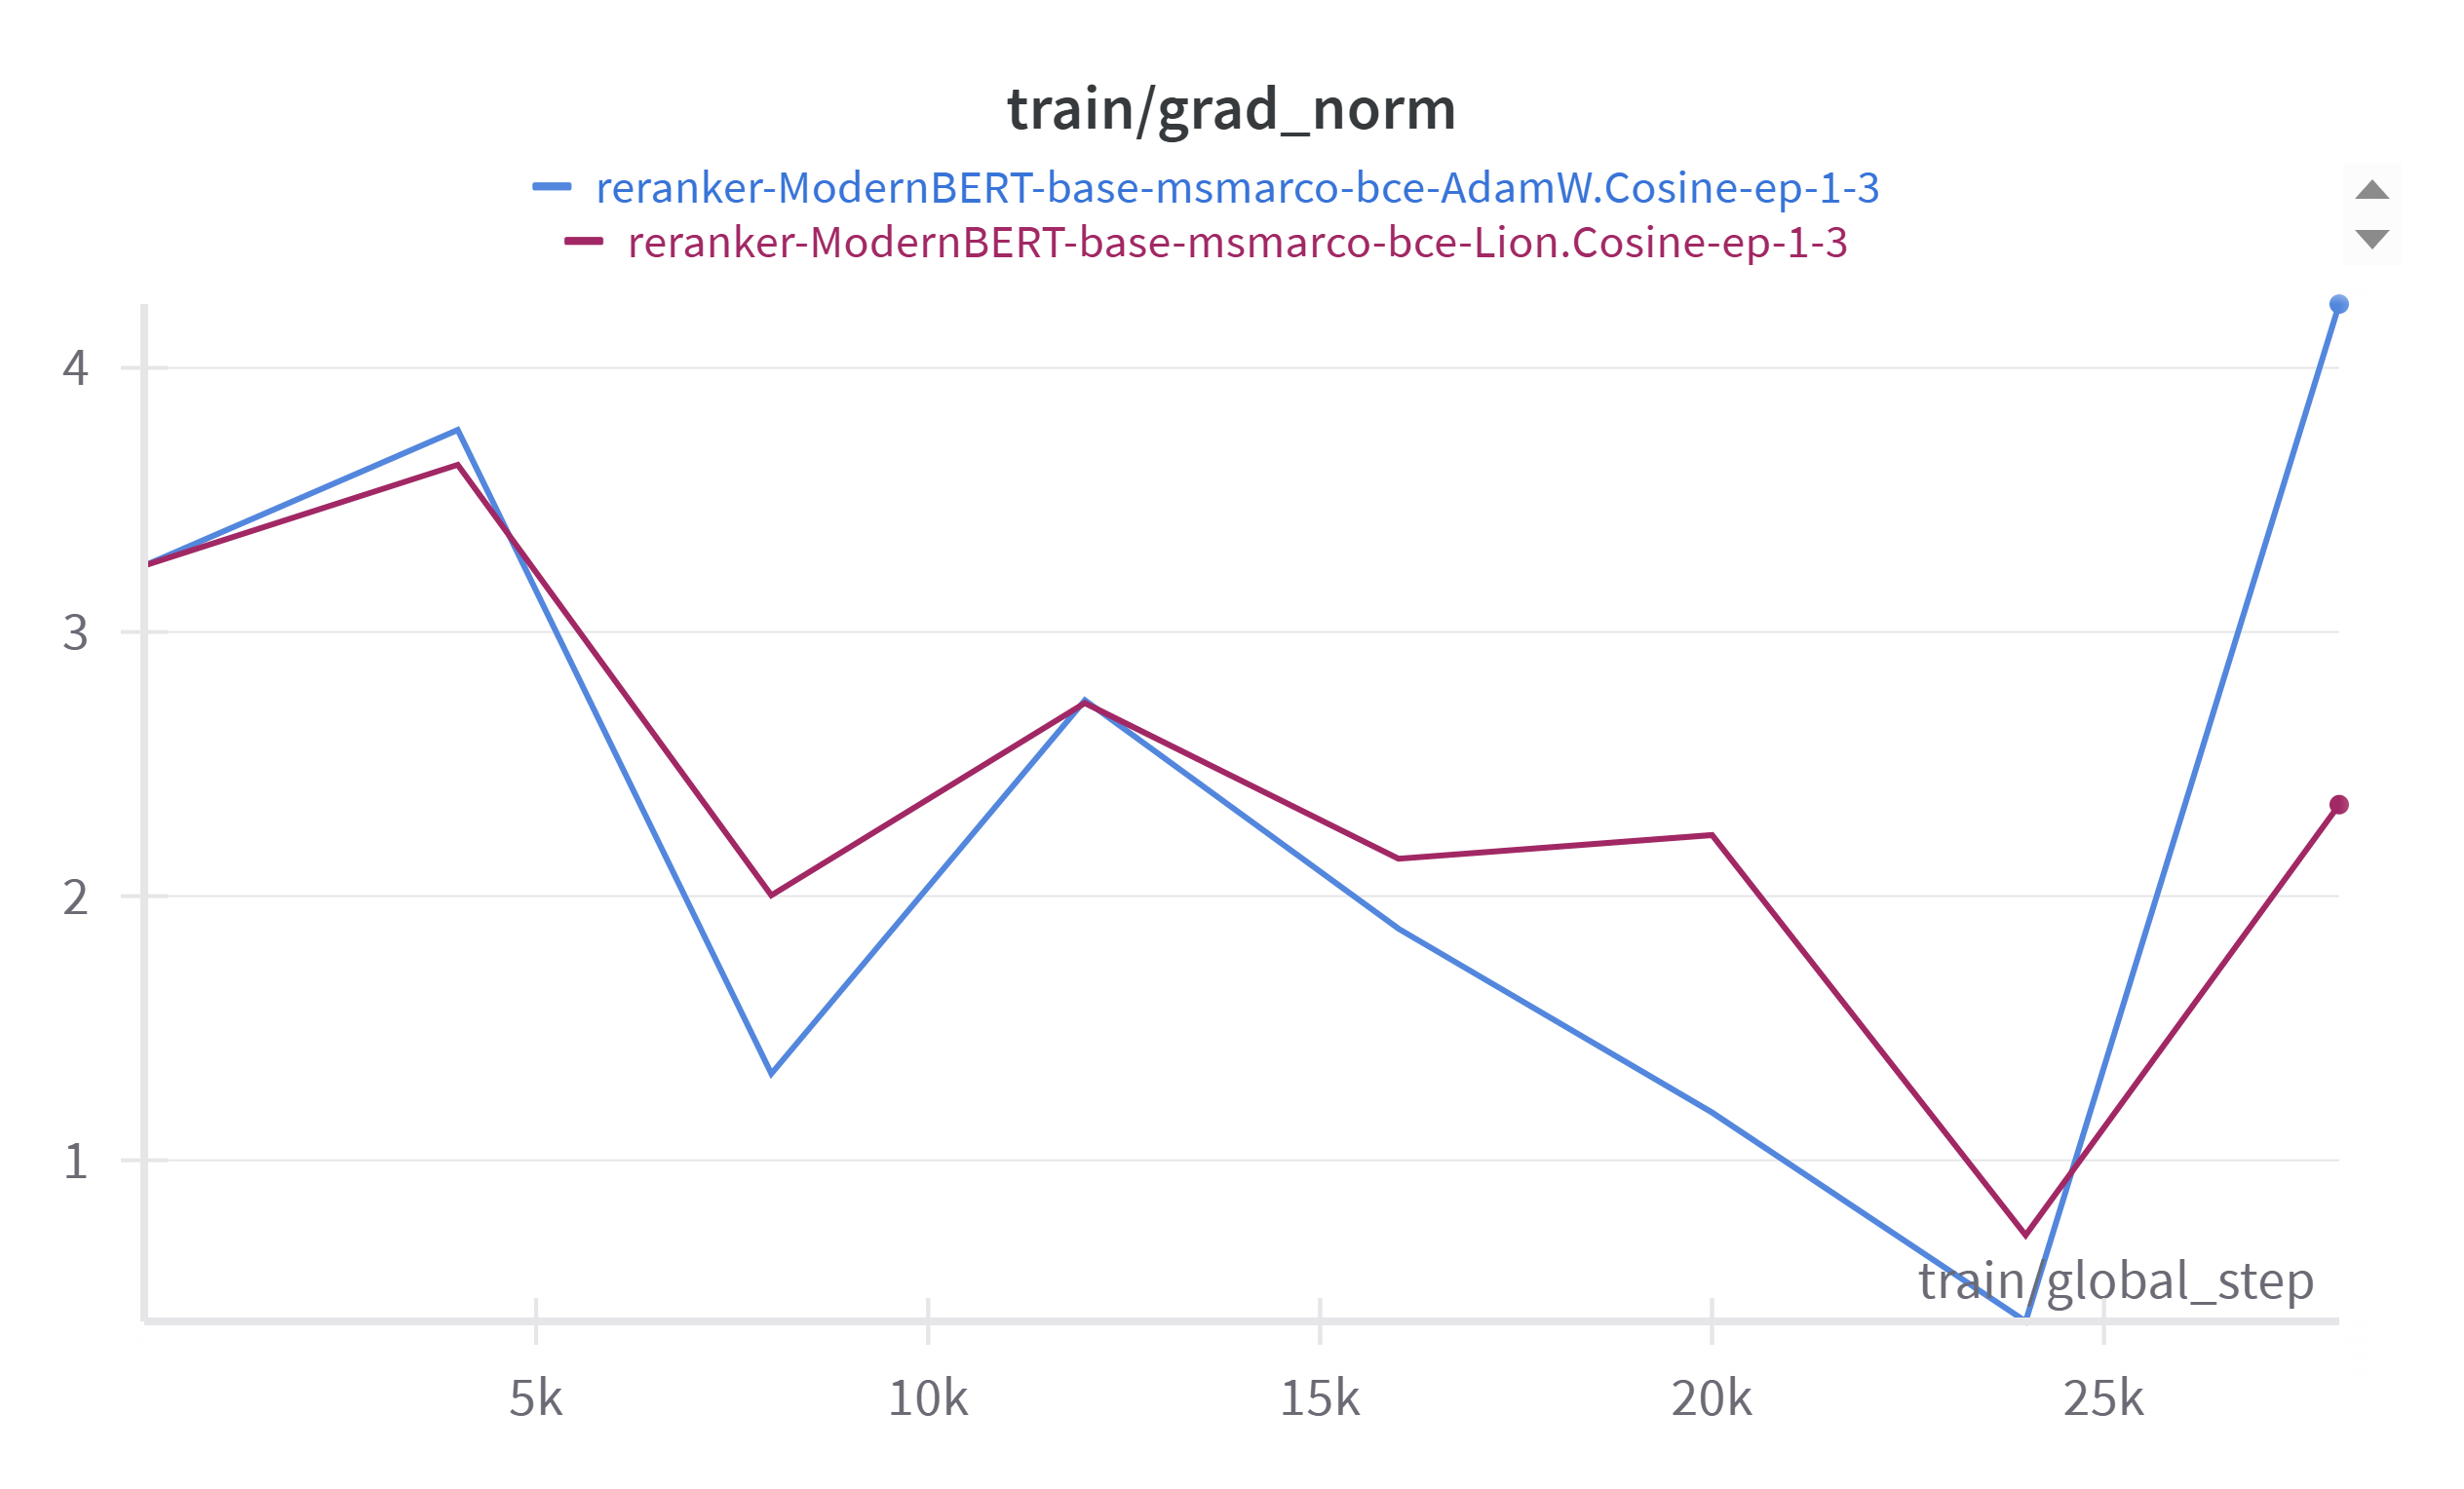
\includegraphics[width=0.8\textwidth]{Figures/modernBERT-Lion-adamW_grad_norm.png}
    \caption{ModernBERT: Gradient Norm Evolution}
    \label{fig:modernbert_grad_norm}
\end{figure}

\subsubsection{GTE Training Dynamics}

\begin{figure}[htbp]
    \centering
    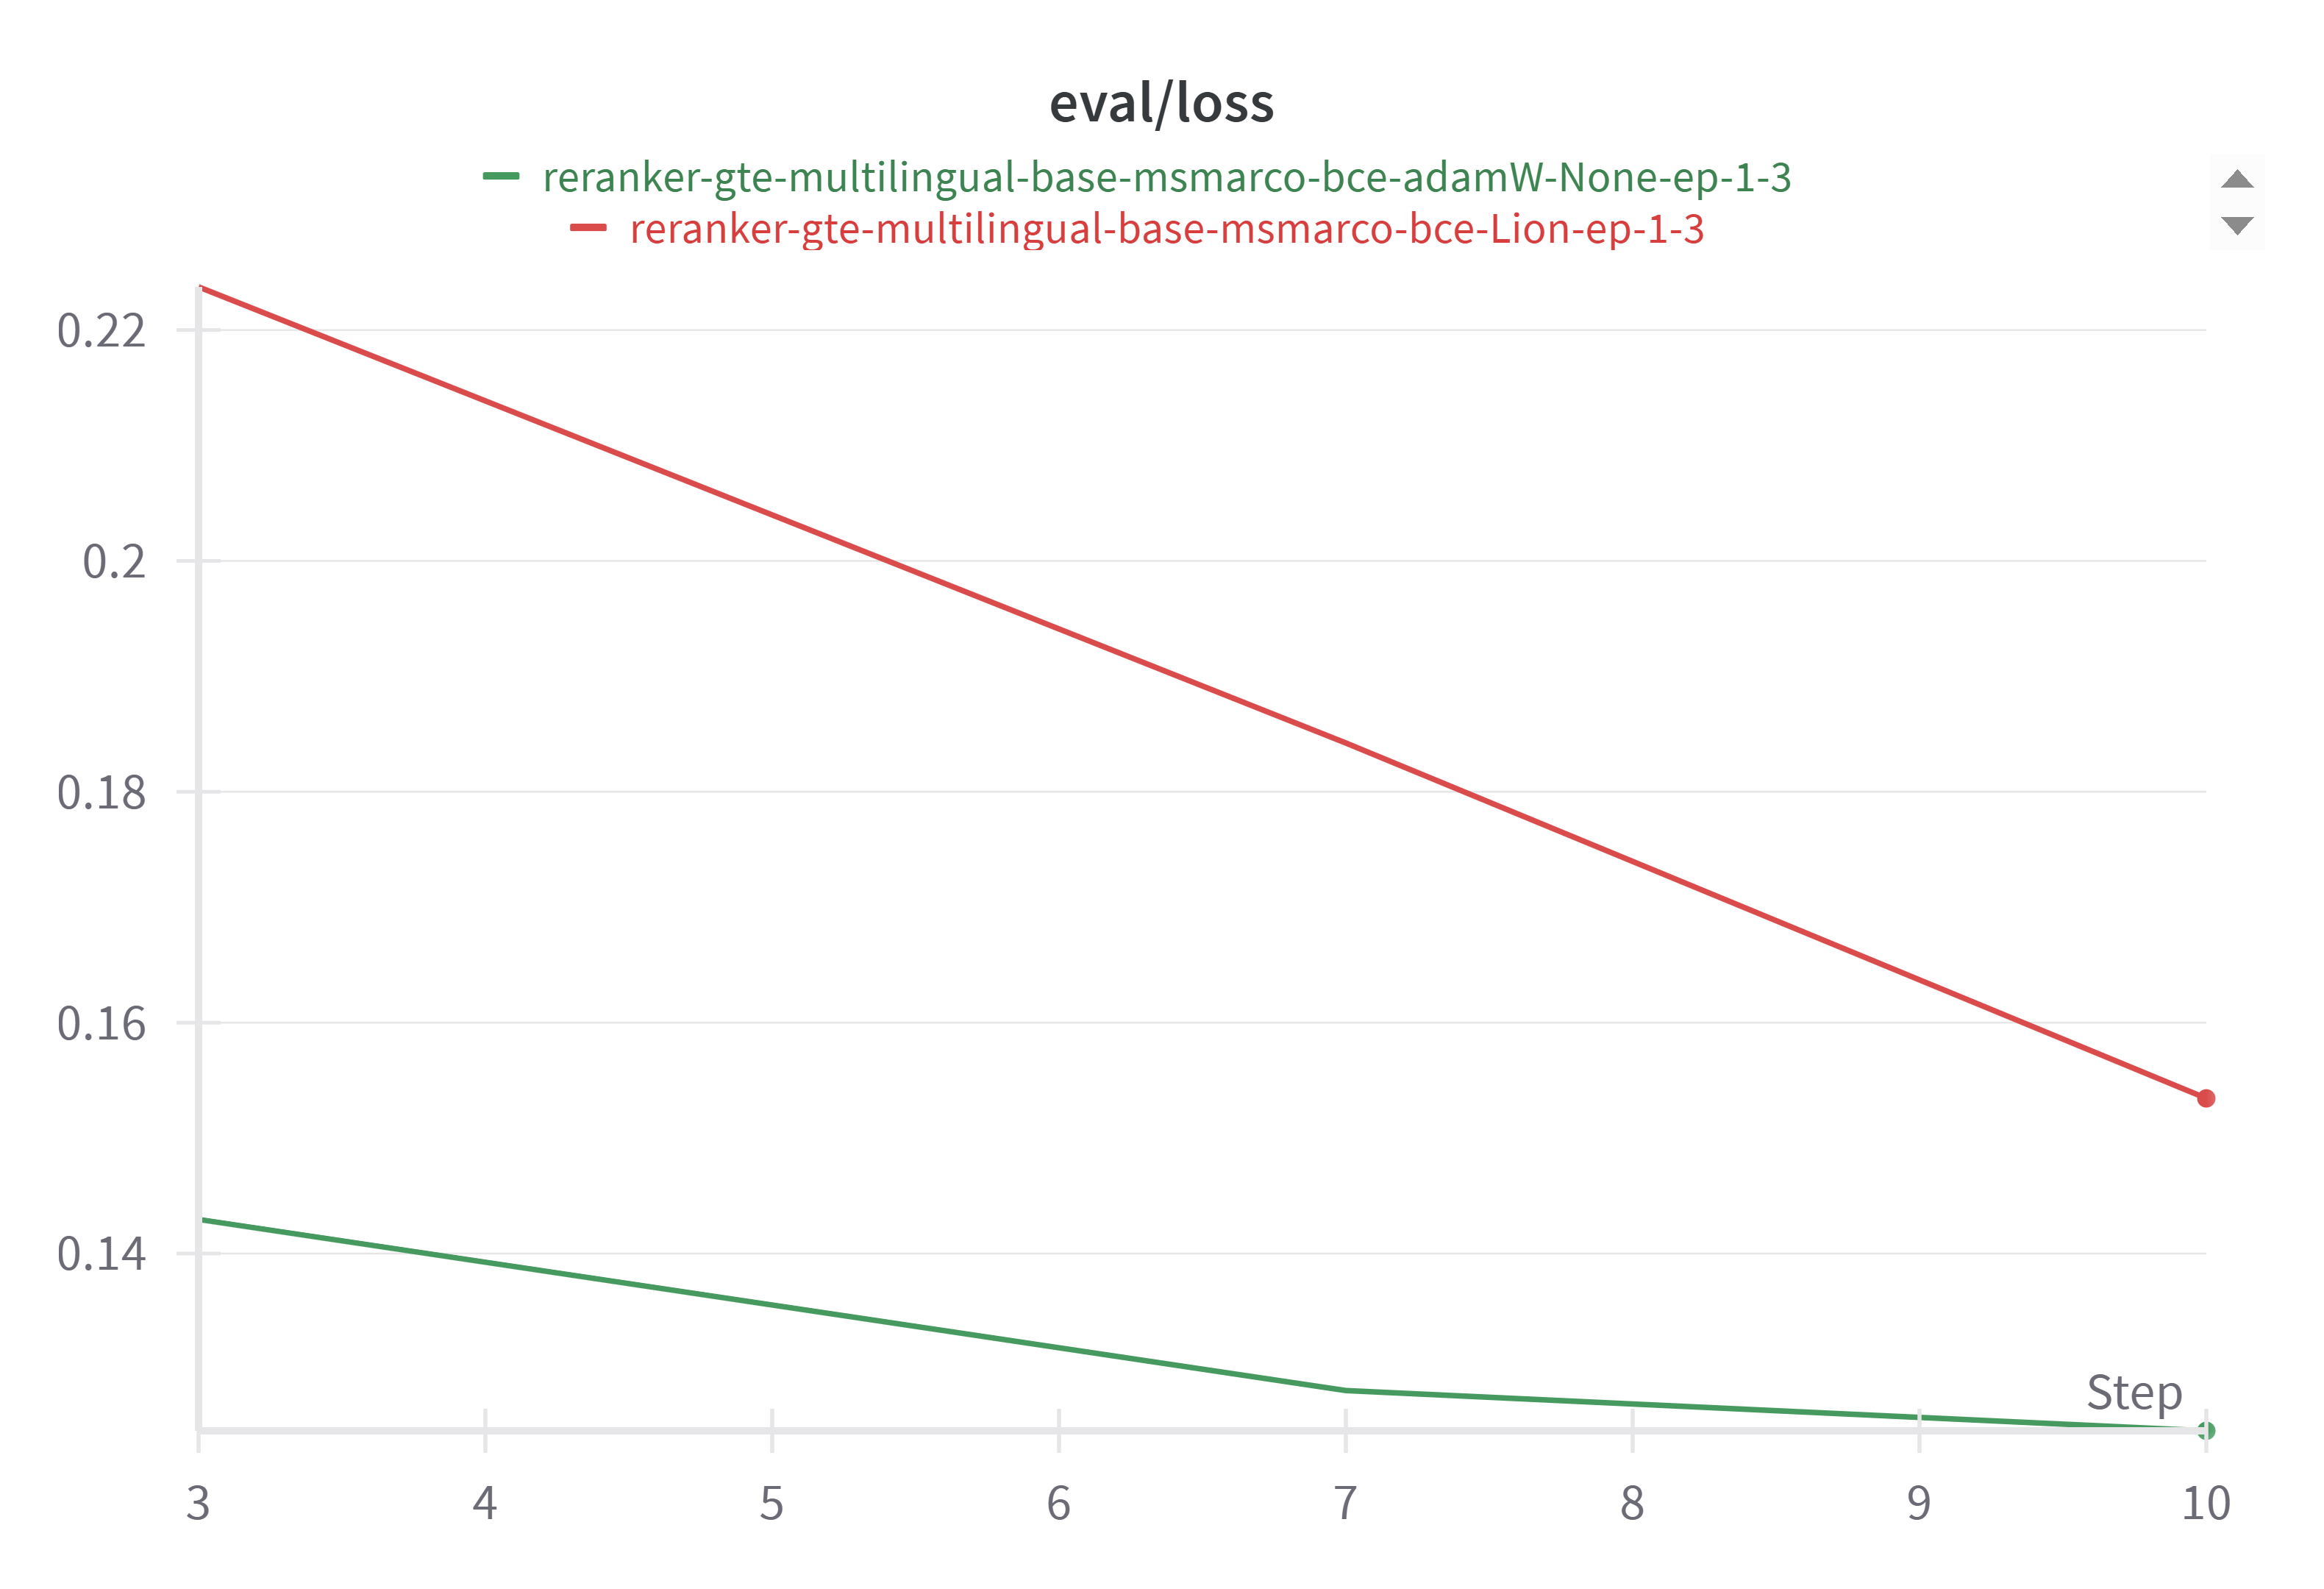
\includegraphics[width=0.8\textwidth]{Figures/gte_adamW_v_lion_eval_loss.png}
    \caption{GTE: Evaluation Loss Comparison}
    \label{fig:gte_eval_loss}
\end{figure}

\begin{figure}[htbp]
    \centering
    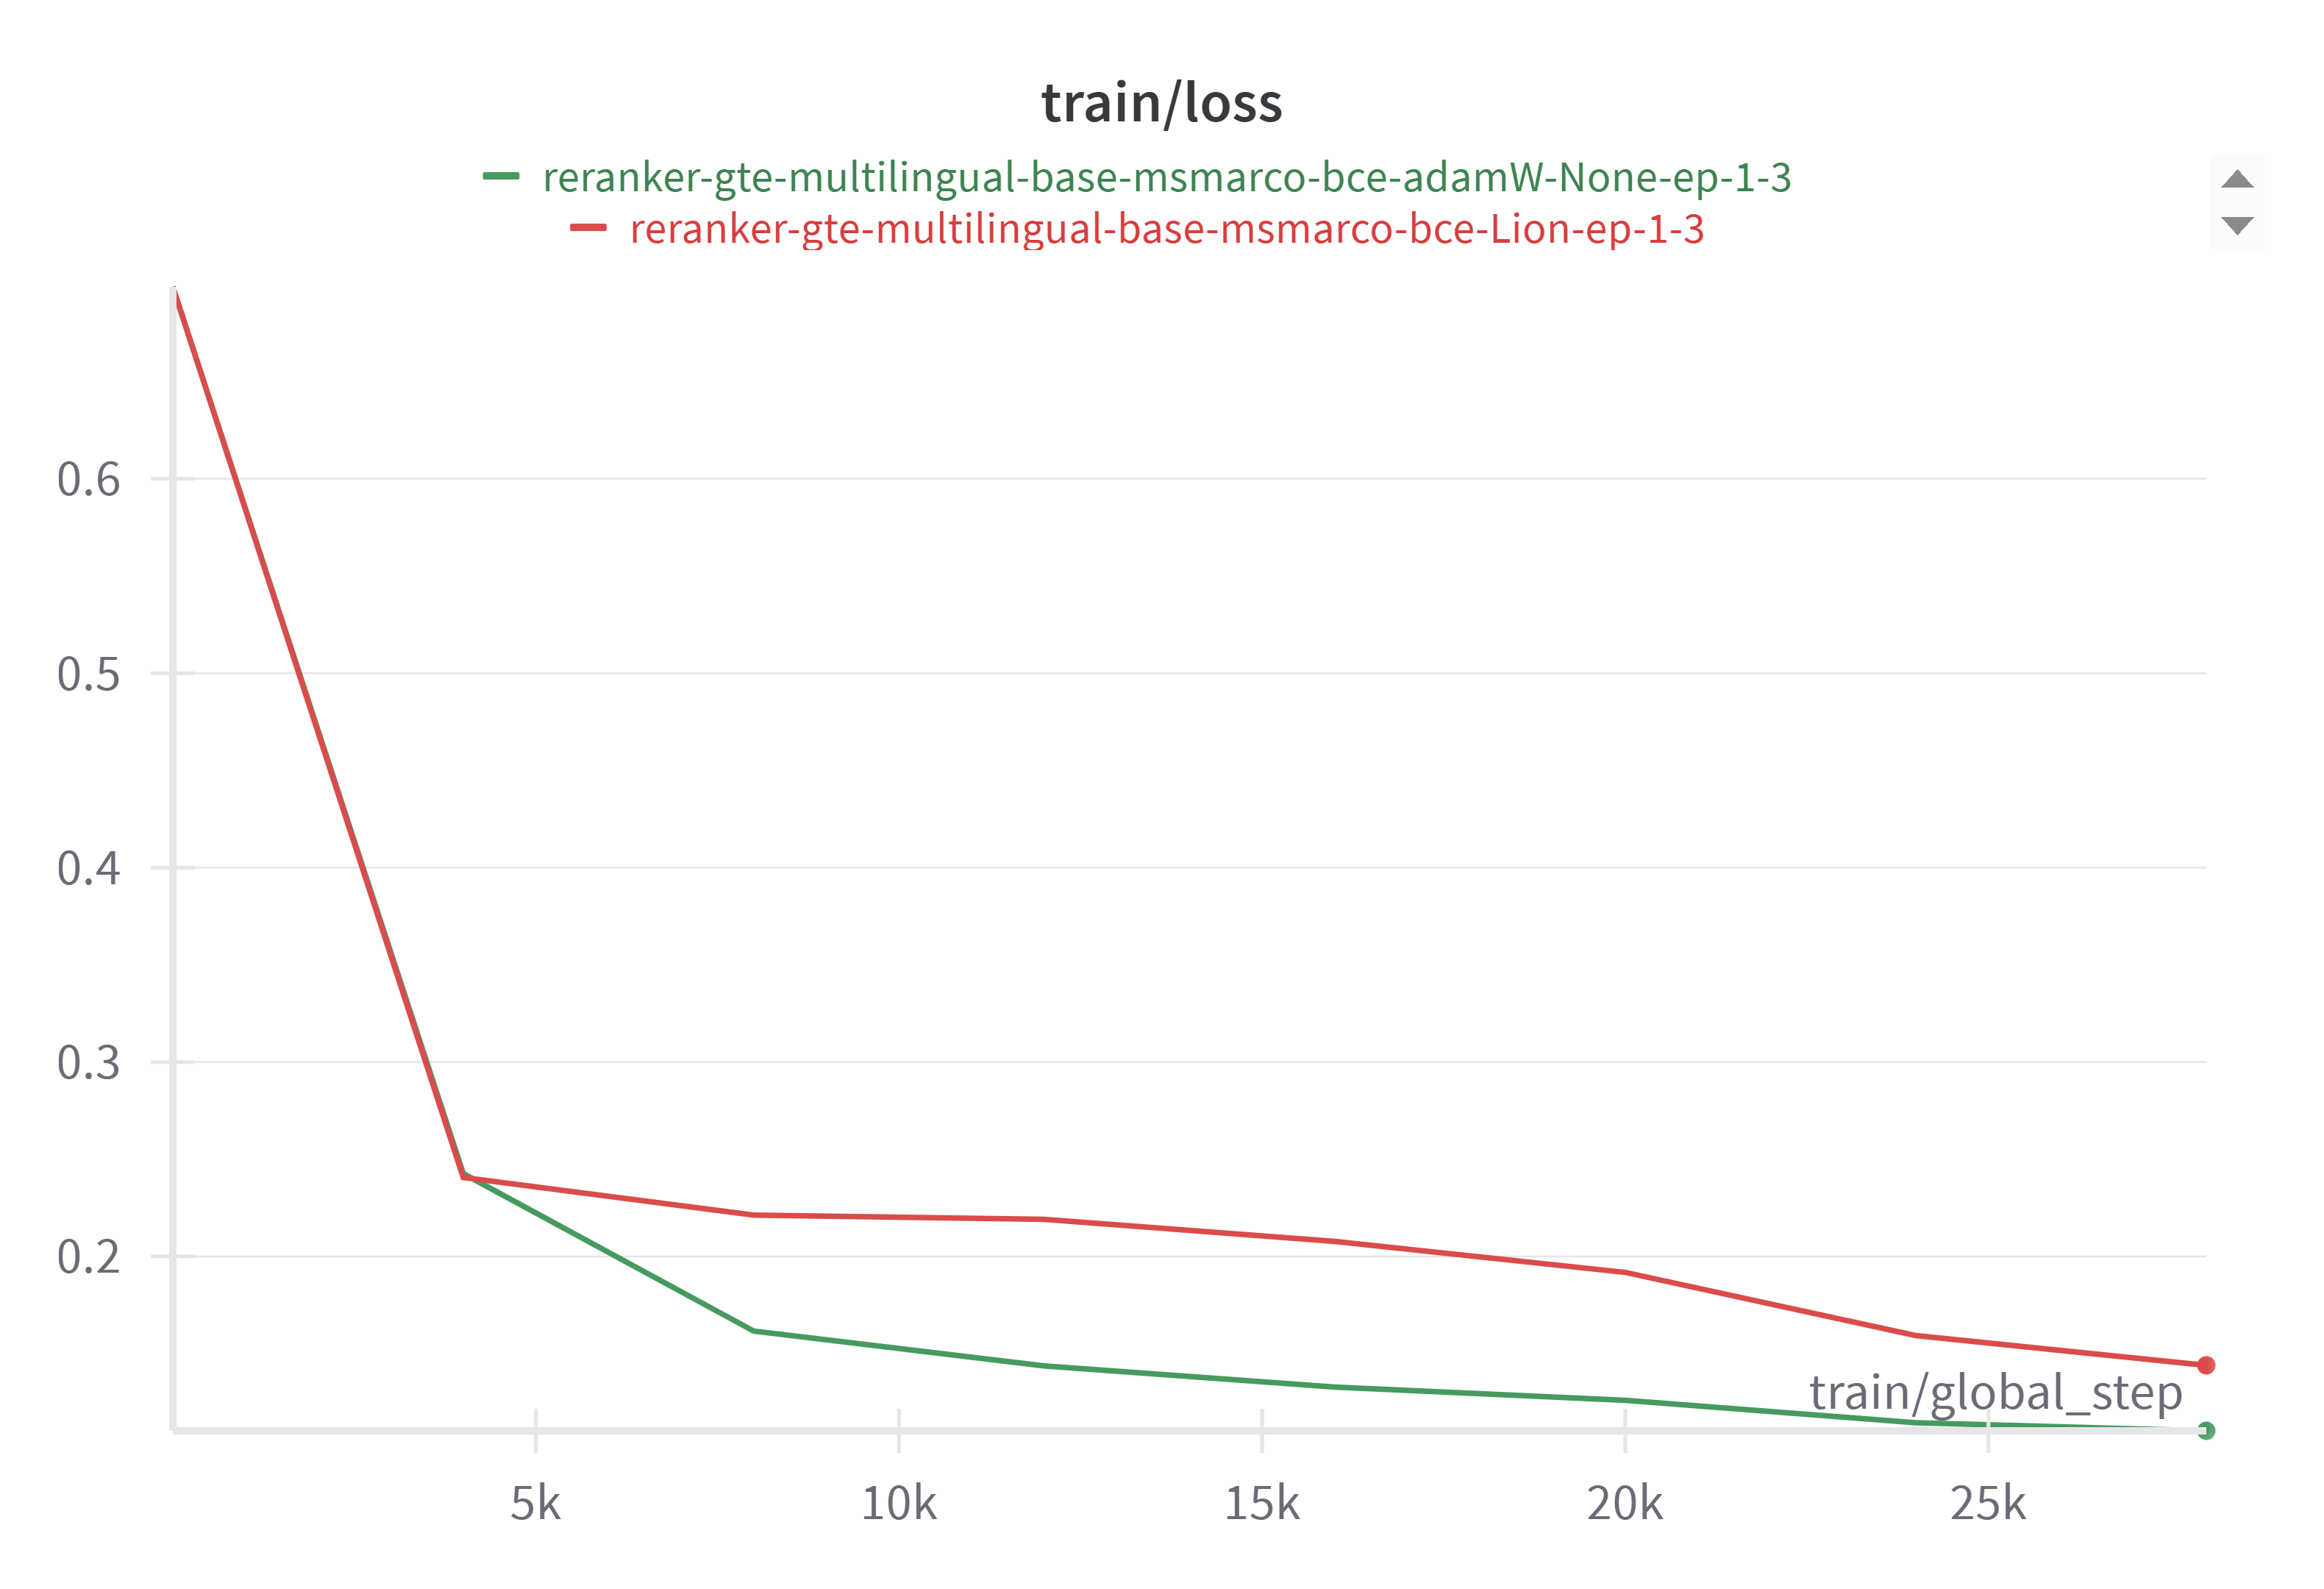
\includegraphics[width=0.8\textwidth]{Figures/gte_adamW_v_lion_train_loss.png}
    \caption{GTE: Training Loss Progression}
    \label{fig:gte_train_loss}
\end{figure}

\begin{figure}[htbp]
    \centering
    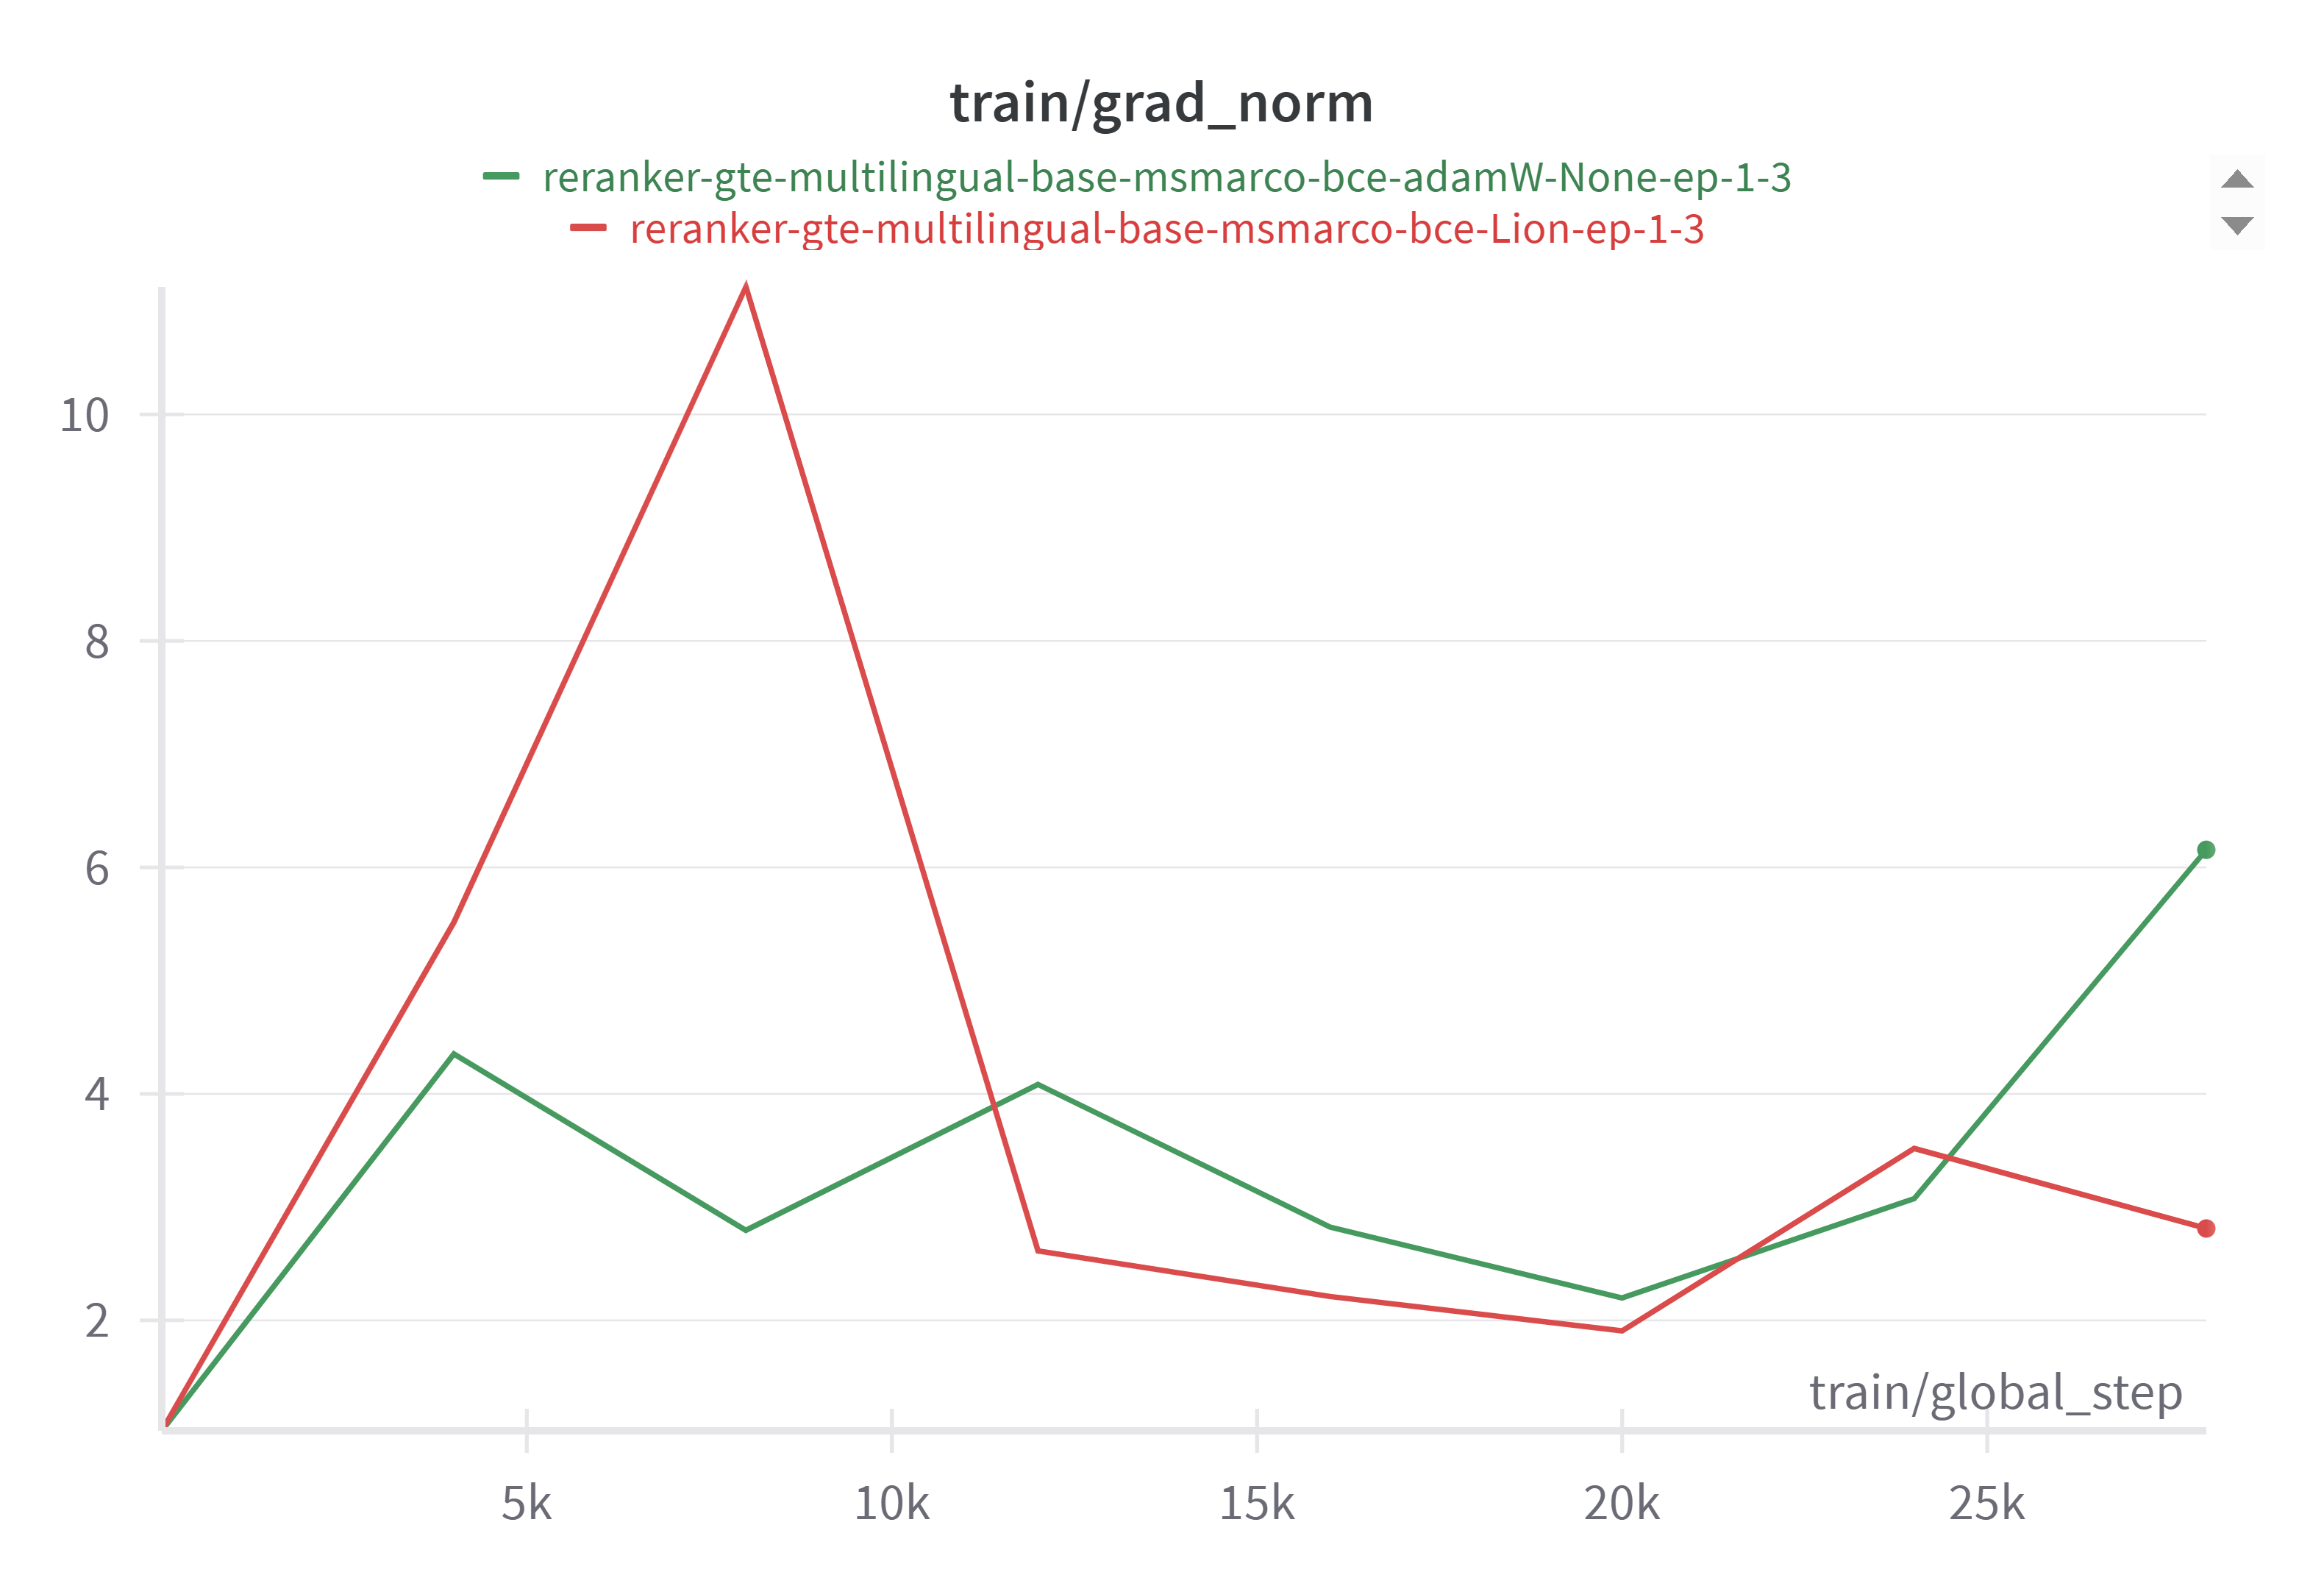
\includegraphics[width=0.8\textwidth]{Figures/gte_adamW_v_lion_grad_norm.png}
    \caption{GTE: Gradient Norm Evolution}
    \label{fig:gte_grad_norm}
\end{figure}

\subsubsection{MiniLM Training Dynamics}

\begin{figure}[htbp]
    \centering
    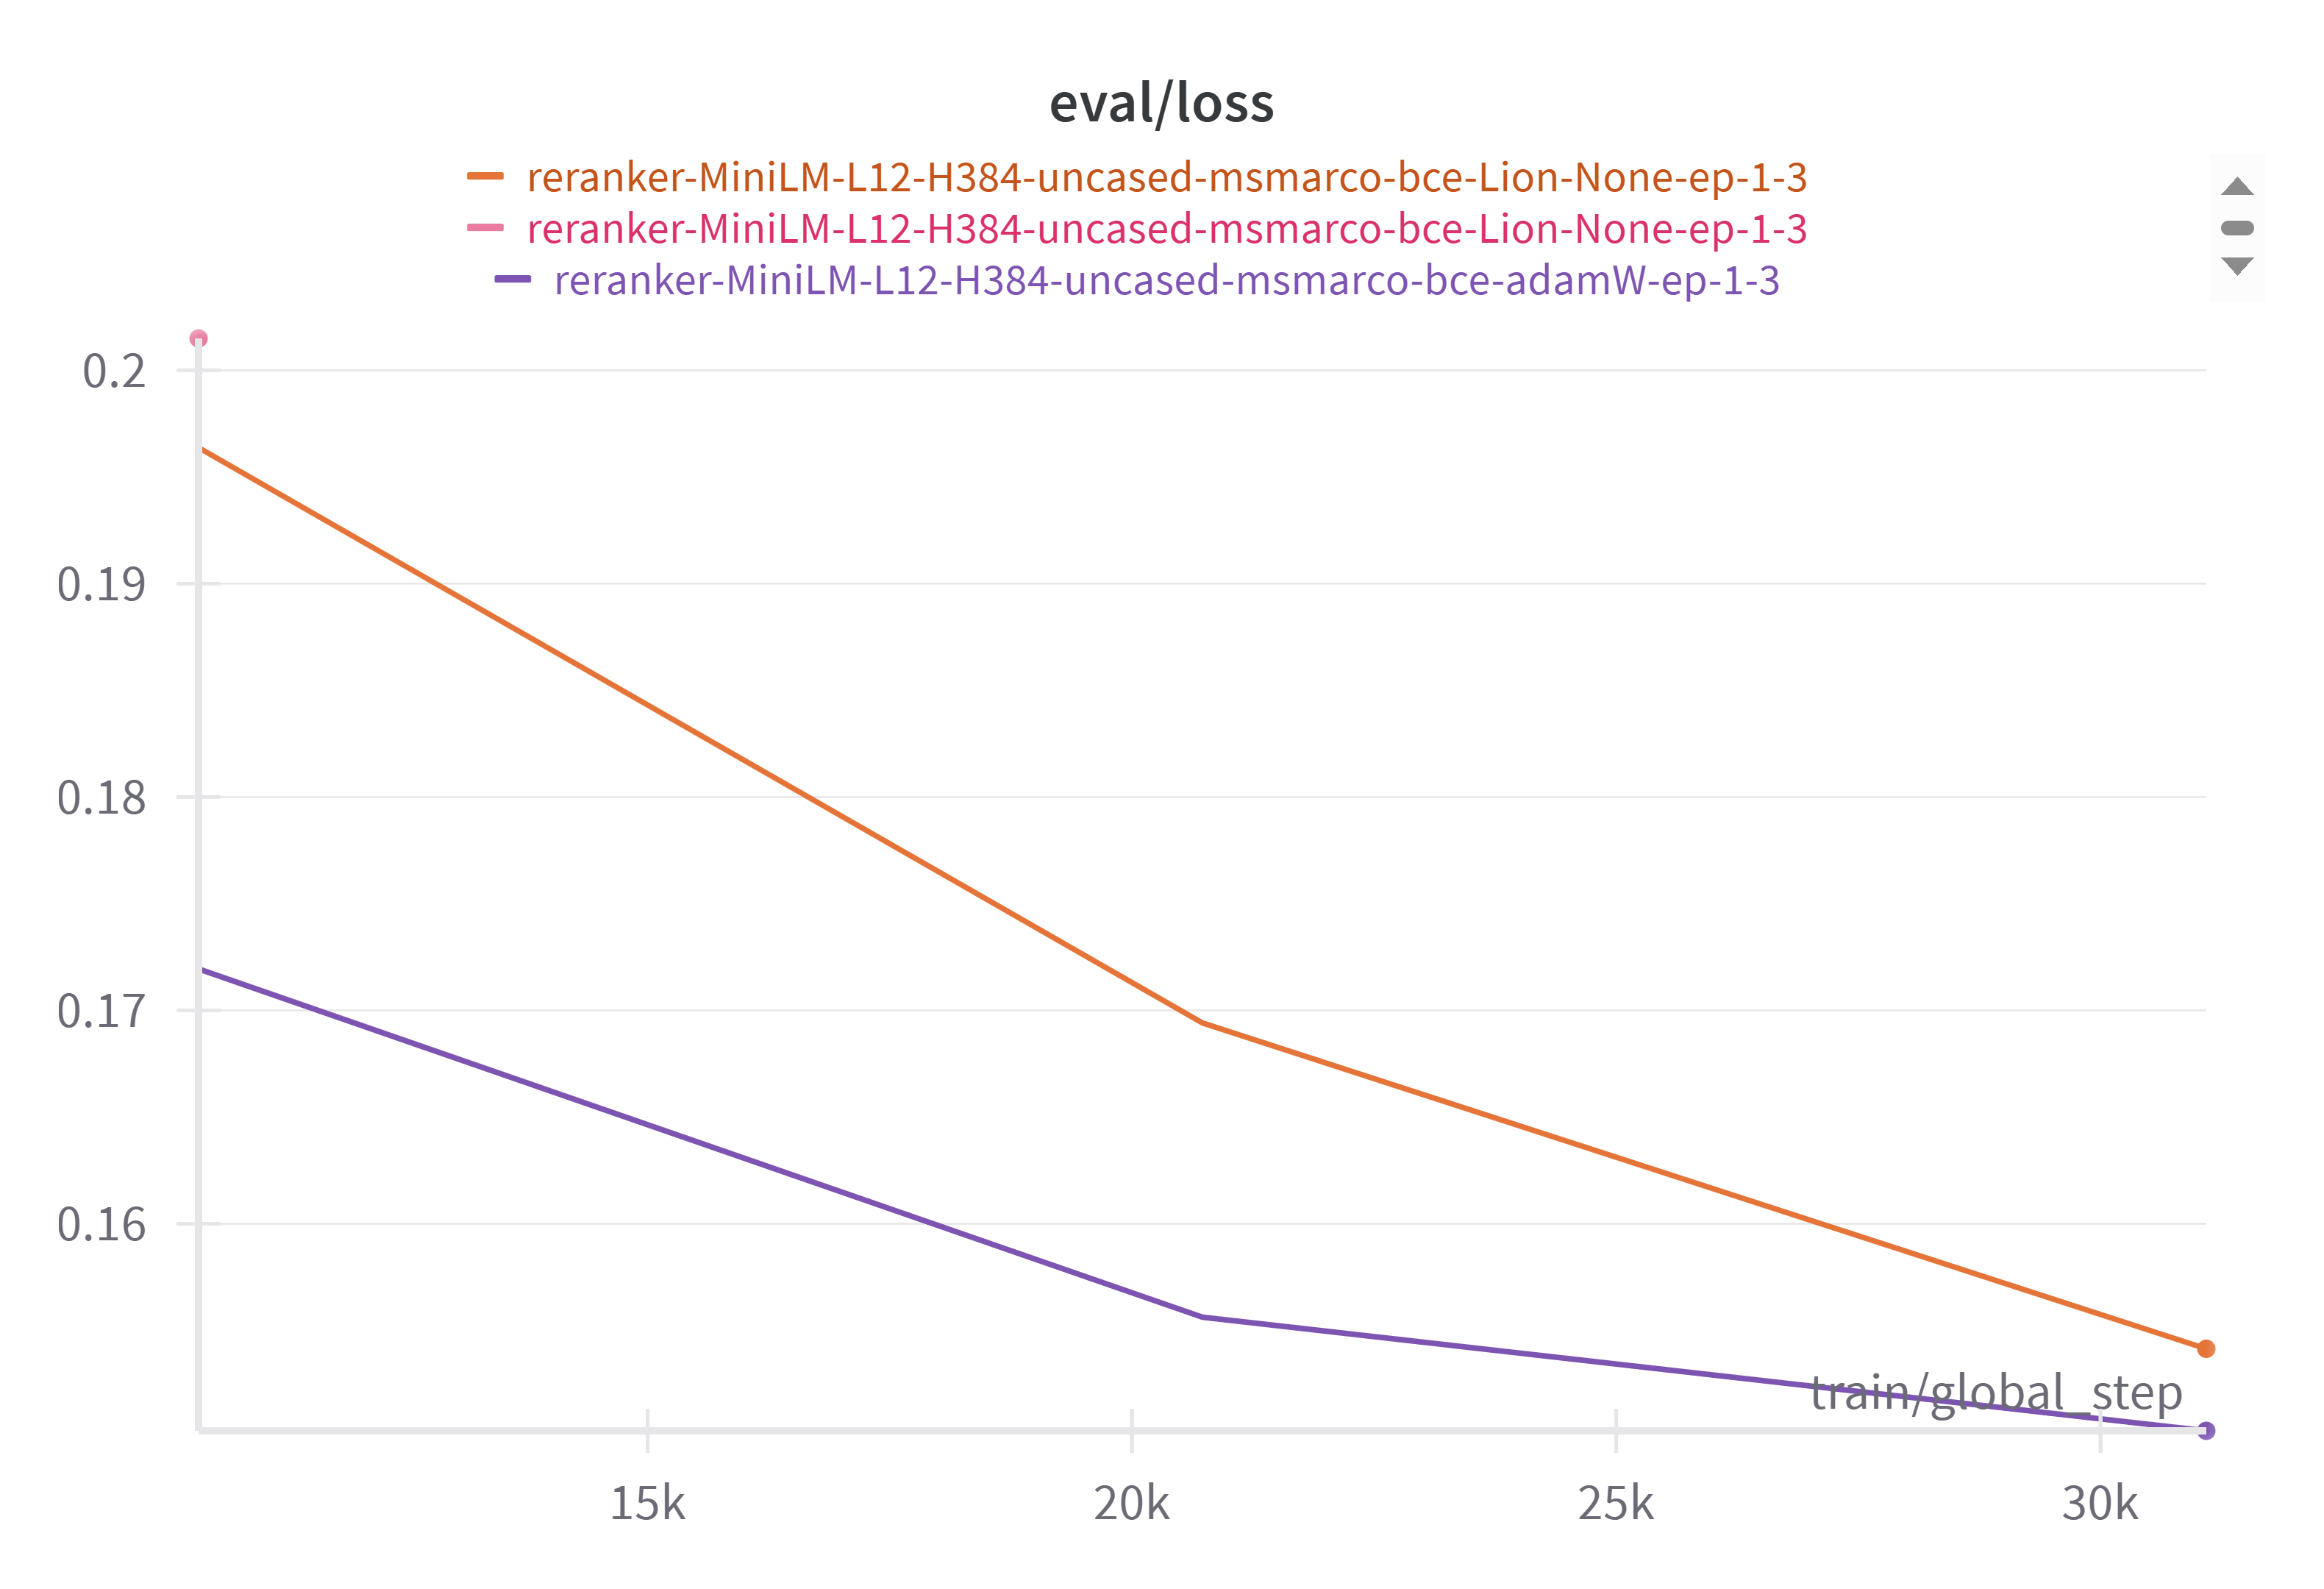
\includegraphics[width=0.8\textwidth]{Figures/microsoft_MiniLM-L12-H384-uncased_adamW_v_Lion_eval_loss.png}
    \caption{MiniLM: Evaluation Loss Comparison}
    \label{fig:minilm_eval_loss}
\end{figure}

\begin{figure}[htbp]
    \centering
    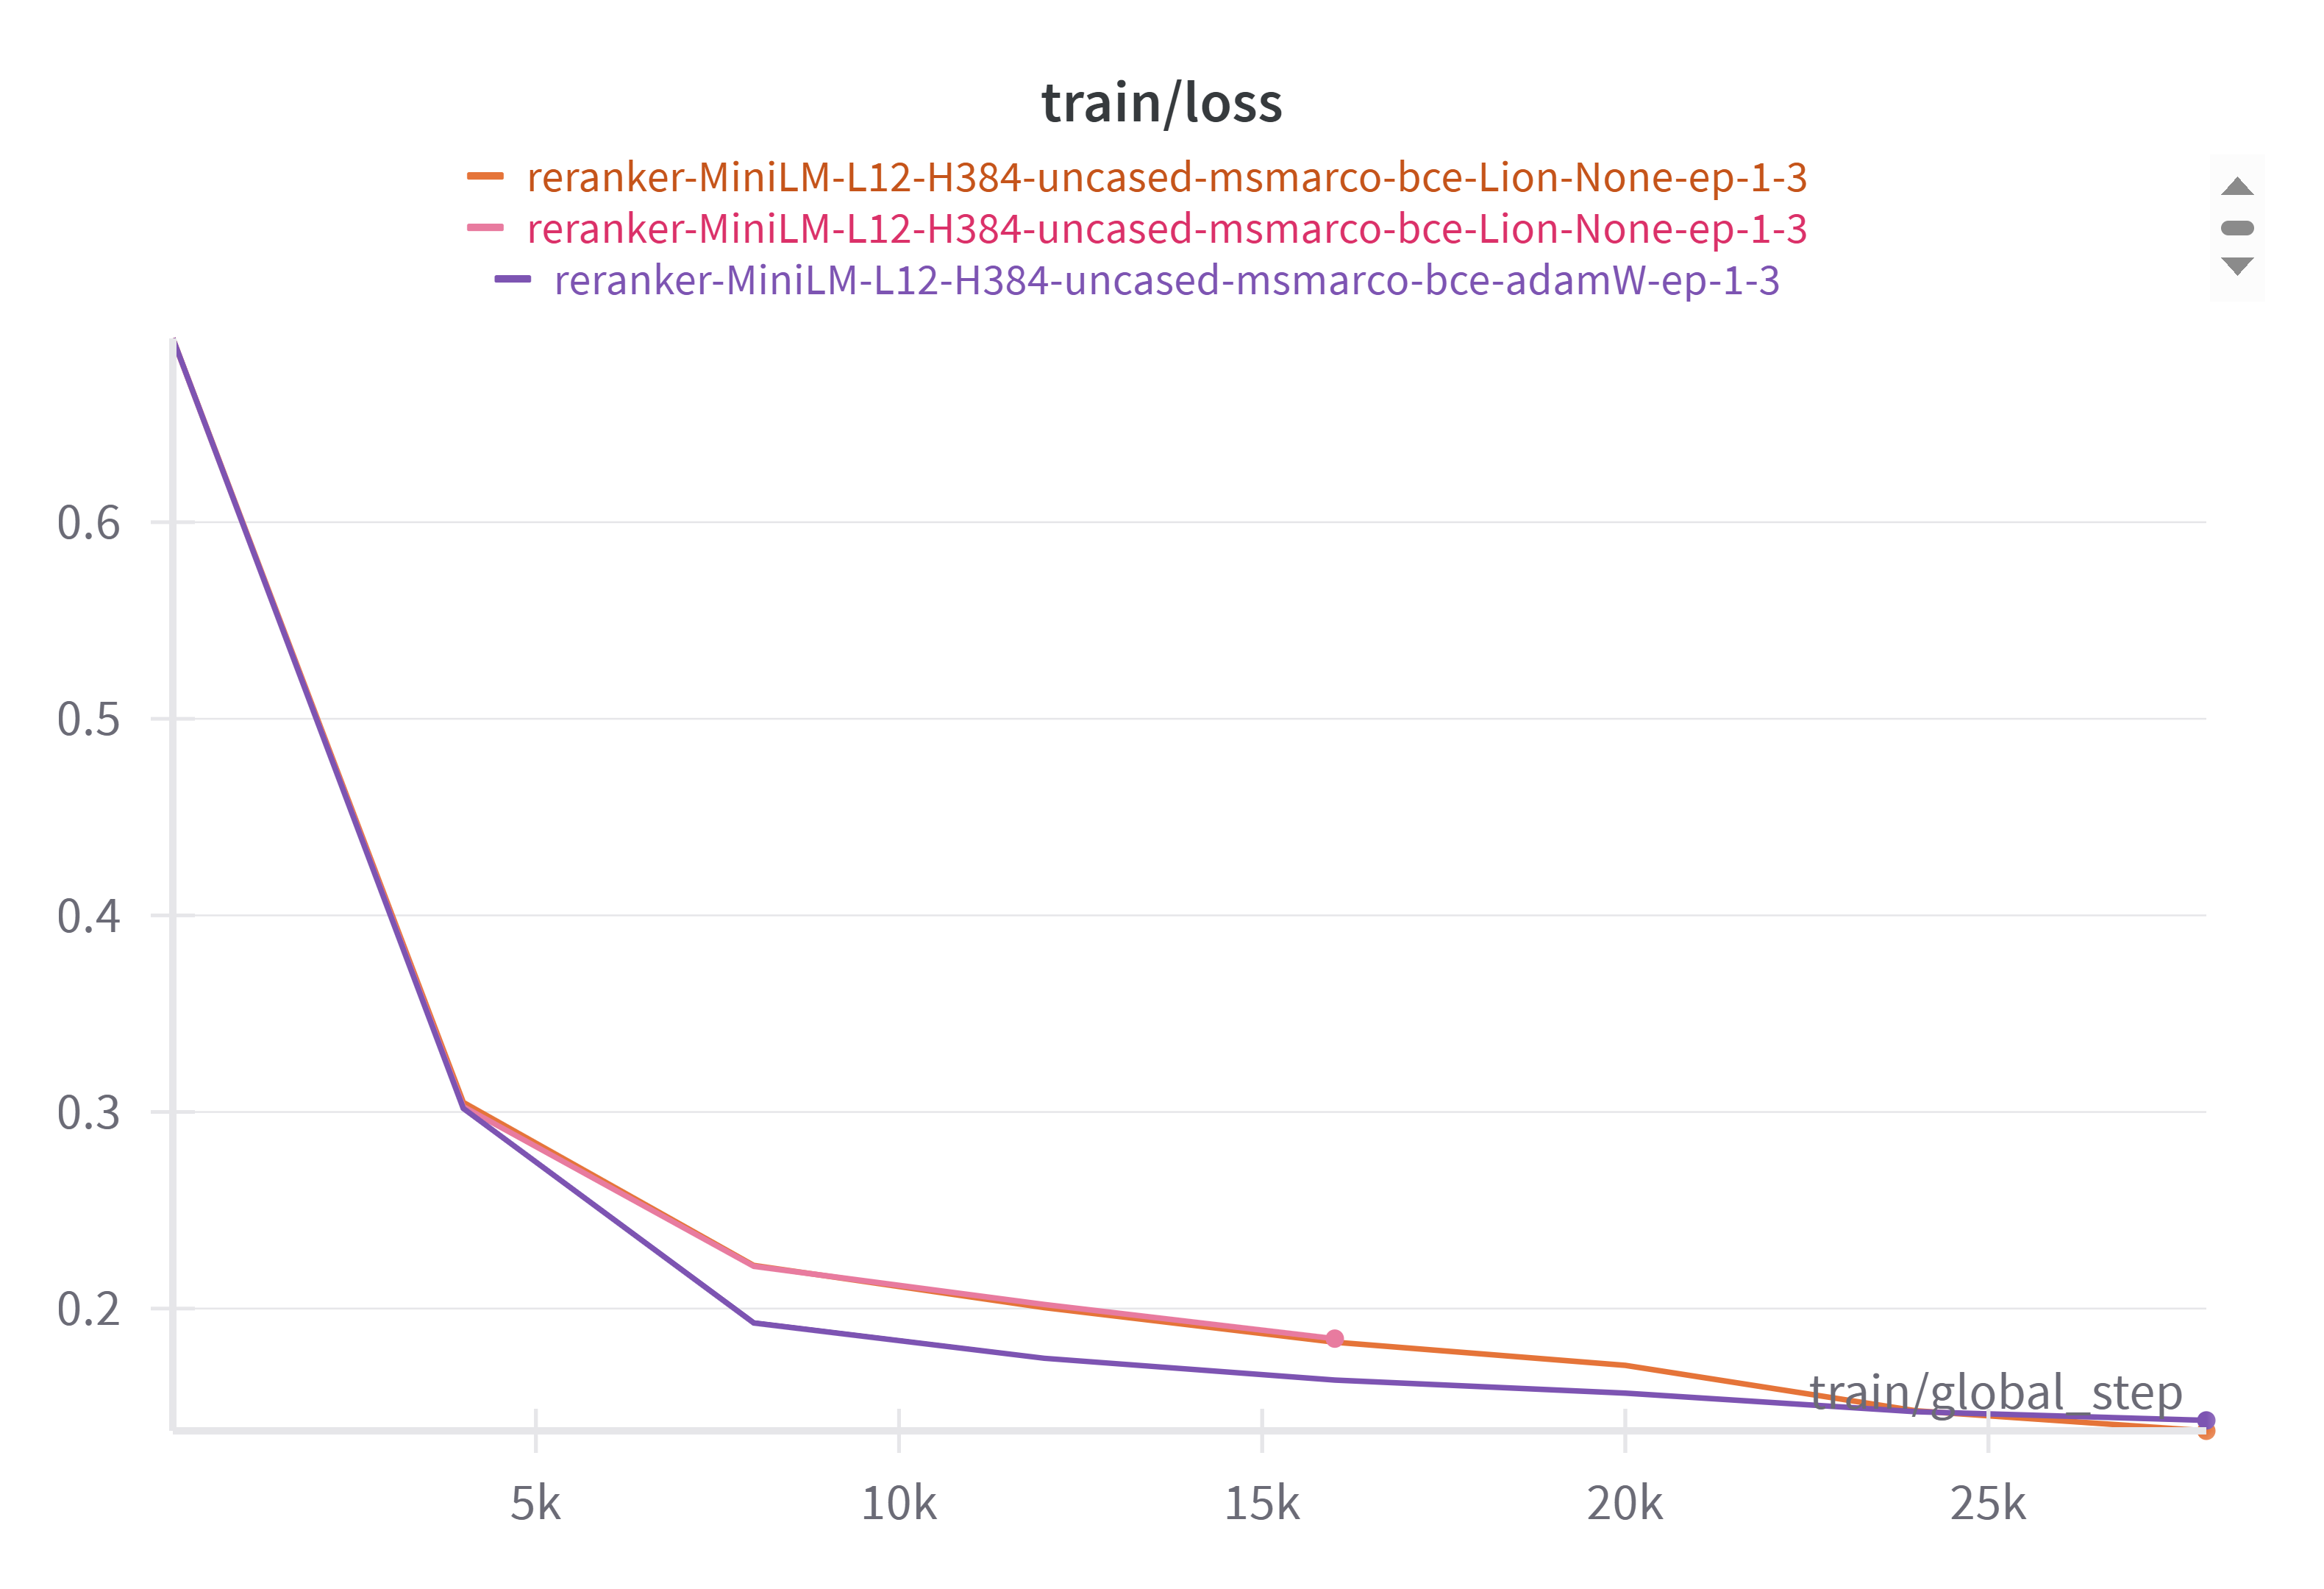
\includegraphics[width=0.8\textwidth]{Figures/microsoft_MiniLM-L12-H384-uncased_adamW_v_Lion_train_loss.png}
    \caption{MiniLM: Training Loss Progression}
    \label{fig:minilm_train_loss}
\end{figure}

\begin{figure}[htbp]
    \centering
    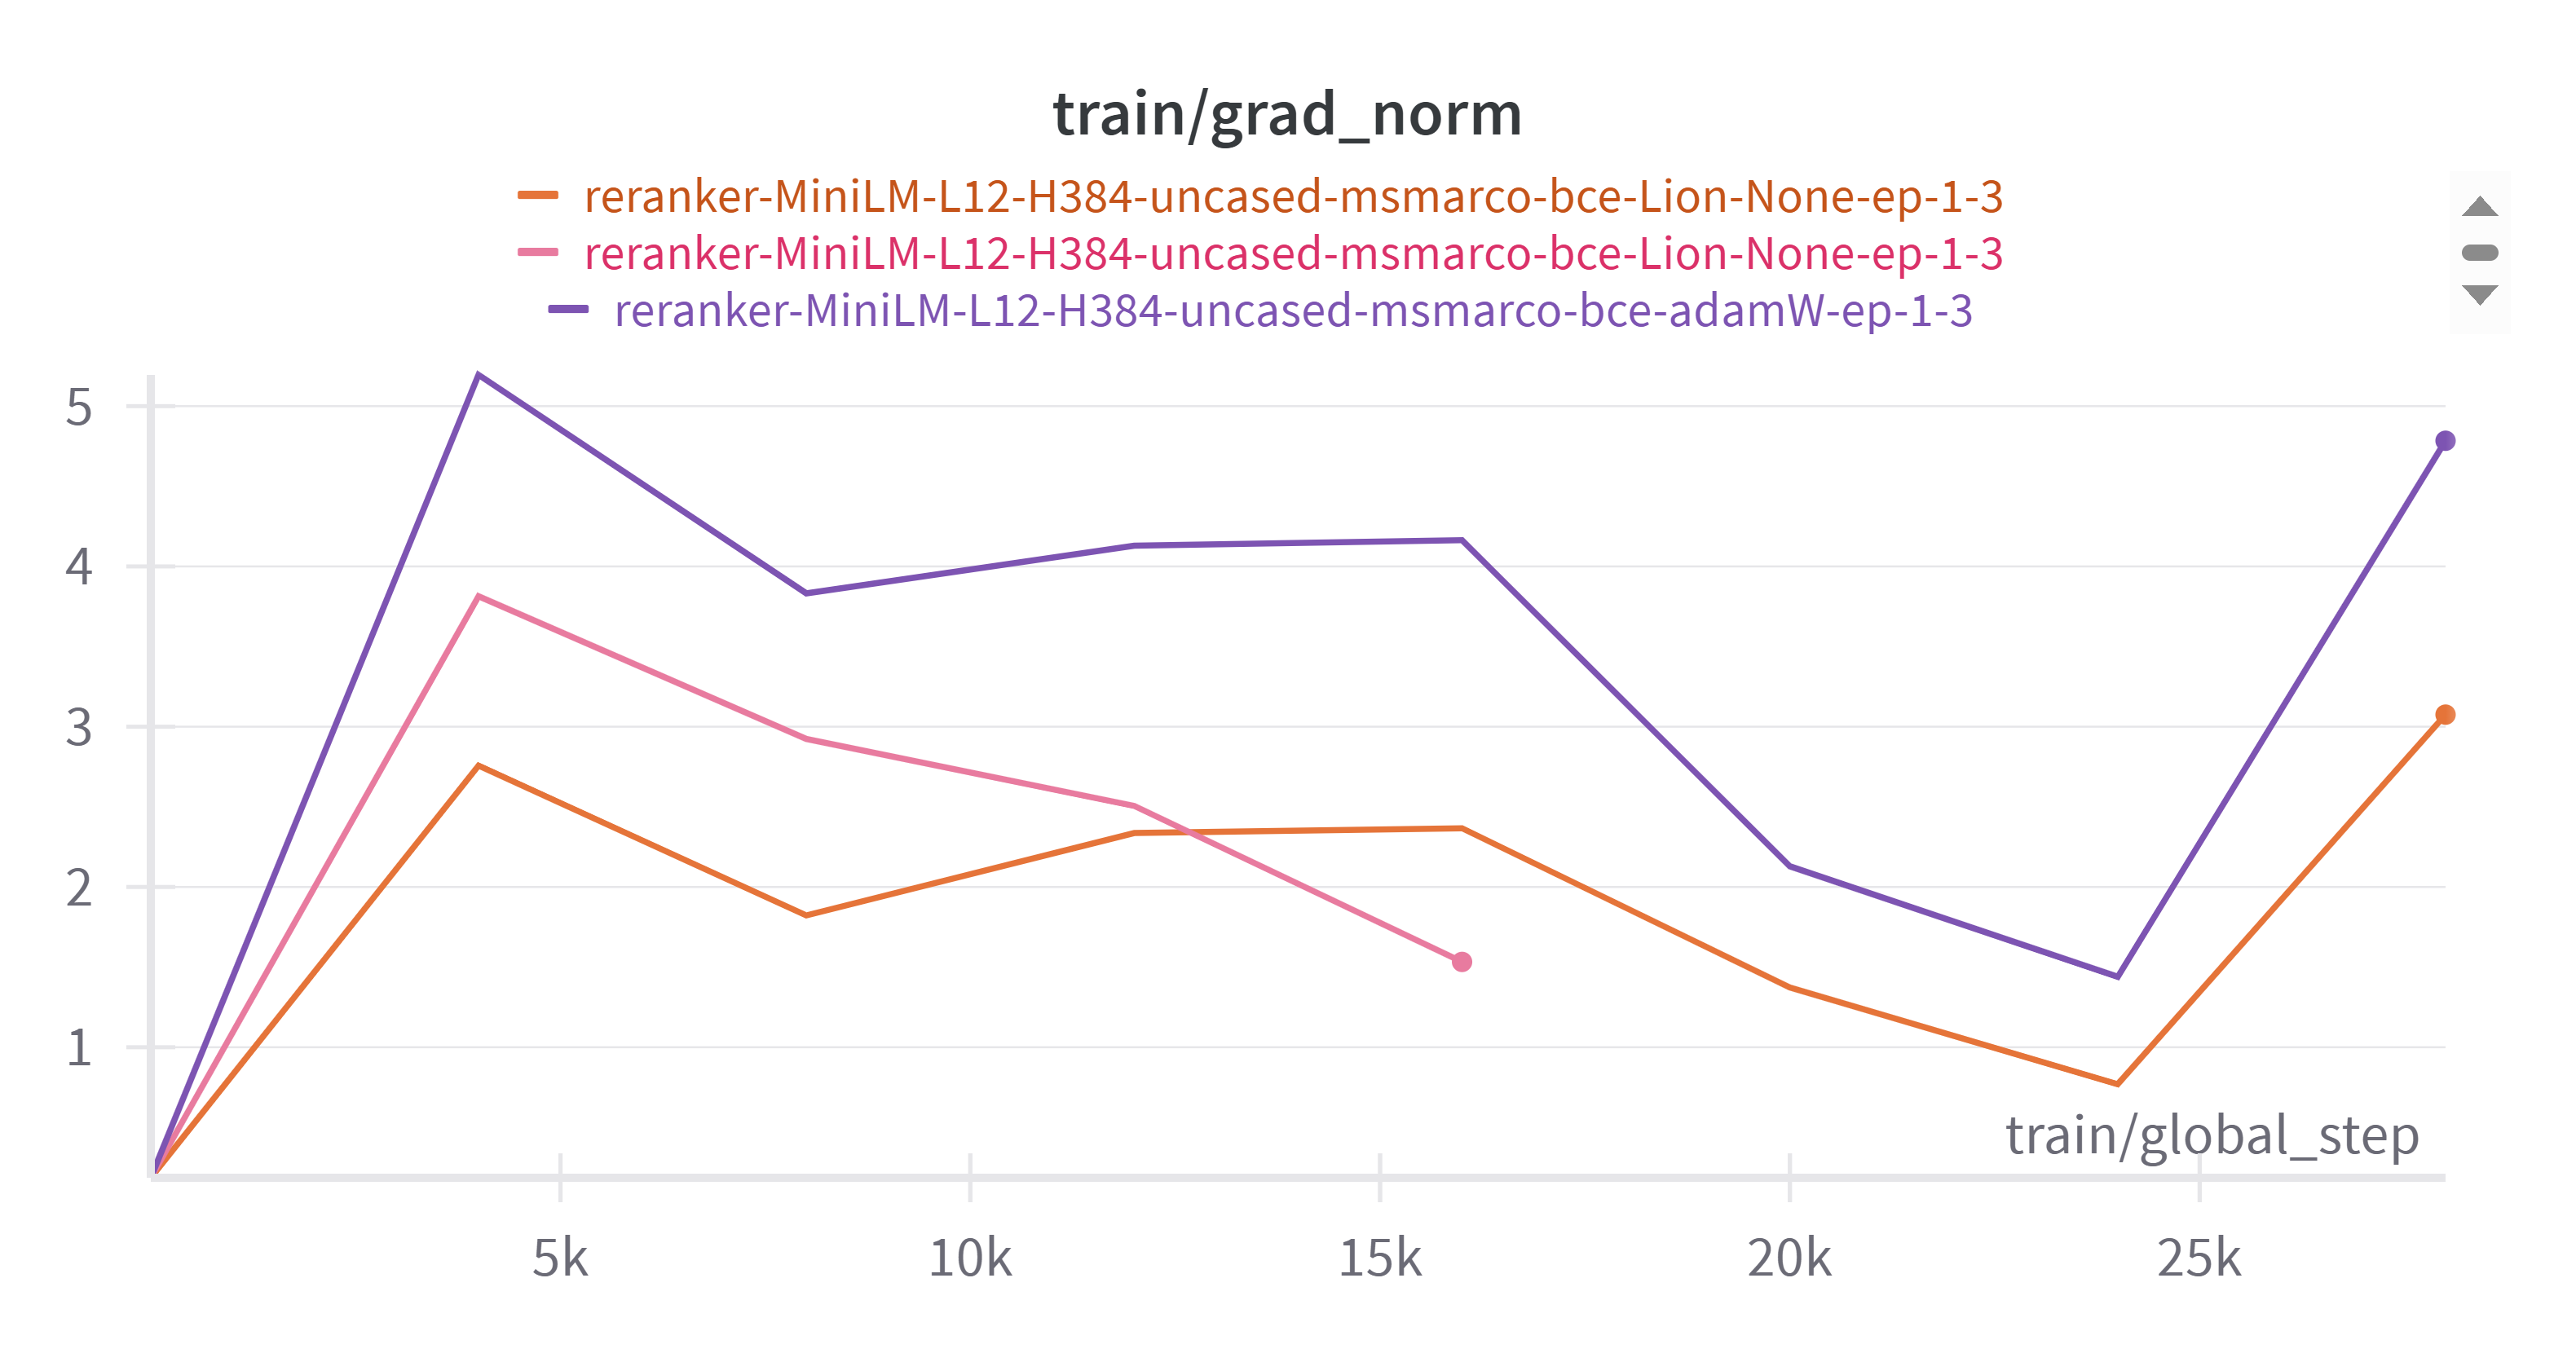
\includegraphics[width=0.8\textwidth]{Figures/microsoft_MiniLM-L12-H384-uncased_adamW_v_Lion_grad_norm.png}
    \caption{MiniLM: Gradient Norm Evolution}
    \label{fig:minilm_grad_norm}
\end{figure}

\section{Discussion of Results}

\subsection{Optimizer Impact Across Models}

The experimental results reveal distinct patterns in how different models interact with the Lion and AdamW optimizers:

\begin{itemize}
    \item \textbf{ModernBERT Performance:} With Lion optimizer and specialized training configuration (lower learning rate of 2e-6 and Cosine Annealing scheduler), ModernBERT achieved the highest overall performance on TREC DL 2019 metrics (NDCG@10: 0.7225, MAP: 0.5115). The training dynamics (Figures \ref{fig:modernbert_eval_loss}-\ref{fig:modernbert_grad_norm}) show more stable convergence with Lion compared to AdamW.
    
    \item \textbf{GTE Behavior:} GTE showed stronger performance with AdamW (NDCG@10: 0.7224) using the standard learning rate (2e-5). The training curves (Figures \ref{fig:gte_eval_loss}-\ref{fig:gte_grad_norm}) indicate that AdamW provided more consistent optimization for this model.
    
    \item \textbf{MiniLM Characteristics:} While MiniLM with AdamW showed better TREC metrics, the Lion optimizer achieved the highest MRR@10 (0.5988) on MS MARCO dev. The training dynamics (Figures \ref{fig:minilm_eval_loss}-\ref{fig:minilm_grad_norm}) suggest that Lion might be particularly effective for certain ranking scenarios.
\end{itemize}

\subsection{Training Dynamics Analysis}

The visualization of training dynamics reveals several key insights:

\begin{itemize}
    \item \textbf{Loss Convergence:} Lion generally shows smoother evaluation loss curves compared to AdamW, particularly evident in the ModernBERT experiments (Figure \ref{fig:modernbert_eval_loss}).
    
    \item \textbf{Gradient Behavior:} The gradient norm plots (Figures \ref{fig:modernbert_grad_norm}, \ref{fig:gte_grad_norm}, \ref{fig:minilm_grad_norm}) show that Lion maintains more consistent gradient magnitudes throughout training.
    
    \item \textbf{Learning Rate Impact:} The Cosine Annealing schedule (Figure \ref{fig:modernbert_lr}) proved particularly effective for ModernBERT with Lion, suggesting that adaptive learning rate strategies can significantly influence optimizer performance.
\end{itemize}

\subsection{Model-Specific Considerations}

The results highlight important model-specific characteristics:

\begin{itemize}
    \item \textbf{Context Length Impact:} Models with longer context capabilities (GTE and ModernBERT, supporting 8192 tokens) generally outperformed MiniLM on TREC DL metrics, suggesting the benefit of extended context for reranking.
    
    \item \textbf{Architecture Influence:} ModernBERT's advanced features (Rotary Positional Embeddings, Flash Attention) appear to synergize well with Lion's optimization approach, particularly with appropriate learning rate scheduling.
    
    \item \textbf{Model Size Considerations:} Despite being smaller, MiniLM showed competitive performance, especially on MRR@10, indicating that model size alone doesn't determine reranking effectiveness.
\end{itemize}

